% Options for packages loaded elsewhere
\PassOptionsToPackage{unicode}{hyperref}
\PassOptionsToPackage{hyphens}{url}
\documentclass[
]{article}
\usepackage{xcolor}
\usepackage{amsmath,amssymb}
\setcounter{secnumdepth}{-\maxdimen} % remove section numbering
\usepackage{iftex}
\ifPDFTeX
  \usepackage[T1]{fontenc}
  \usepackage[utf8]{inputenc}
  \usepackage{textcomp} % provide euro and other symbols
\else % if luatex or xetex
  \usepackage{unicode-math} % this also loads fontspec
  \defaultfontfeatures{Scale=MatchLowercase}
  \defaultfontfeatures[\rmfamily]{Ligatures=TeX,Scale=1}
\fi
\usepackage{lmodern}
\ifPDFTeX\else
  % xetex/luatex font selection
\fi
% Use upquote if available, for straight quotes in verbatim environments
\IfFileExists{upquote.sty}{\usepackage{upquote}}{}
\IfFileExists{microtype.sty}{% use microtype if available
  \usepackage[]{microtype}
  \UseMicrotypeSet[protrusion]{basicmath} % disable protrusion for tt fonts
}{}
\makeatletter
\@ifundefined{KOMAClassName}{% if non-KOMA class
  \IfFileExists{parskip.sty}{%
    \usepackage{parskip}
  }{% else
    \setlength{\parindent}{0pt}
    \setlength{\parskip}{6pt plus 2pt minus 1pt}}
}{% if KOMA class
  \KOMAoptions{parskip=half}}
\makeatother
\usepackage{longtable,booktabs,array}
\newcounter{none} % for unnumbered tables
\usepackage{calc} % for calculating minipage widths
% Correct order of tables after \paragraph or \subparagraph
\usepackage{etoolbox}
\makeatletter
\patchcmd\longtable{\par}{\if@noskipsec\mbox{}\fi\par}{}{}
\makeatother
% Allow footnotes in longtable head/foot
\IfFileExists{footnotehyper.sty}{\usepackage{footnotehyper}}{\usepackage{footnote}}
\makesavenoteenv{longtable}
\usepackage{graphicx}
\makeatletter
\newsavebox\pandoc@box
\newcommand*\pandocbounded[1]{% scales image to fit in text height/width
  \sbox\pandoc@box{#1}%
  \Gscale@div\@tempa{\textheight}{\dimexpr\ht\pandoc@box+\dp\pandoc@box\relax}%
  \Gscale@div\@tempb{\linewidth}{\wd\pandoc@box}%
  \ifdim\@tempb\p@<\@tempa\p@\let\@tempa\@tempb\fi% select the smaller of both
  \ifdim\@tempa\p@<\p@\scalebox{\@tempa}{\usebox\pandoc@box}%
  \else\usebox{\pandoc@box}%
  \fi%
}
% Set default figure placement to htbp
\def\fps@figure{htbp}
\makeatother
\setlength{\emergencystretch}{3em} % prevent overfull lines
\providecommand{\tightlist}{%
  \setlength{\itemsep}{0pt}\setlength{\parskip}{0pt}}
\usepackage{bookmark}
\IfFileExists{xurl.sty}{\usepackage{xurl}}{} % add URL line breaks if available
\urlstyle{same}
% fallback for those not using the hyperref driver hyperxmp:
\makeatletter
\@ifundefined{xmpquote}{\newcommand{\xmpquote}[1]{#1}}{}
\makeatother
\hypersetup{
  hidelinks,
  pdfcreator={LaTeX via pandoc}}

\author{}
\date{}

\begin{document}

\section{Effects of Observing a Robot Expressing Approach-Avoidance
Conflict on Observers' Self-Evaluations of Personal
Courage}\label{effects-of-observing-a-robot-expressing-approach-avoidance-conflict-on-observers-self-evaluations-of-personal-courage}

Yuki Shimizu1,*, Midori Ban2, Hideyuki Takahashi3, Hiroshi Ishiguro1

1Department of Engineering Science, Osaka University, Osaka, Japan

2Kyoto Tachibana University, Kyoto, Japan

3Faculty of Science and Engineering, Otemon Gakuin University, Osaka,
Japan

\textbf{* Correspondence:}Yuki
Shimizusimizu.yuki@irl.sys.es.osaka-u.ac.jp

\textbf{Word count: 6,254}

\textbf{Number of figures and tables: 7 figures and 5 tables}

\textbf{Keywords:} personal courage, approach-avoidance conflict,
observational learning, human-robot interaction, internal state, robot
expression, observer responses.

\subsection{Abstract}\label{abstract}

Courage involves pursuing a valued action despite fear, hesitation, or
competing motives. However, the pre-action conflict relevant to judging
an act as courageous is difficult to observe directly and manipulate
systematically when another human serves as the model. Robots provide a
means of representing such otherwise covert motives in a controlled and
reproducible form. We therefore examined how a robot's expression of
approach-avoidance conflict is perceived and how it relates to
observers' immediate self-evaluations of personal courage. Speech
bubbles were projected near the head of a cylindrical robot to present
approach and avoidance motives in a scenario in which the robot
encountered a person littering in a park. Study 1 compared conflict and
no-conflict conditions and sequential and simultaneous presentation
methods to determine whether a robot expressing approach-avoidance
conflict was perceived as courageous. Study 2 varied whether the robot
expressed one motive direction or both approach and avoidance motives
and whether it admonished the litterer, and examined whether
post-stimulus courage self-evaluations differed according to observers'
preexisting courage tendency. In Study 1, the conflict condition yielded
higher courage and conflict ratings than the no-conflict condition. In
Study 2, the predicted three-way interaction was not supported. Instead,
we observed a significant two-way interaction between preexisting
courage tendency group and conflict expression that was not specified in
the primary hypothesis. The low-courage group showed a marginal trend
toward higher self-evaluations in the conflict condition, whereas the
high-courage group reported significantly lower self-evaluations in the
conflict condition. Admonishing behavior had no clear effect. This
contrasting pattern suggests that robot-expressed conflict may be
received differently depending on observers' preexisting courage
tendency. The study provides a controlled HRI paradigm for examining how
robot-expressed motives are perceived and highlights the importance of
considering user characteristics when designing robots that display cues
to internal processes.

\subsection{Introduction}\label{introduction}

In everyday life, people sometimes must pursue valued actions even when
those actions involve fear or anxiety. In this study, we refer to this
capacity as personal courage. Courage has been conceptualized not as the
absence of fear but as moving toward meaningful action in the presence
of fear (Rachman, 1984; Woodard and Pury, 2007). Personal courage is
important because it situates the difficulty of an action within the
actor's own context. Pury et al.~(2007) distinguished between general
courage, which is evaluated as courageous by most people, and personal
courage, which is courageous in light of a person's life context and
personal constraints. From this perspective, a child with a learning
disability going to school on the day of a major test, or a person
wrapping Christmas presents for the first time after being unable to do
so for many years because of a history of post-traumatic stress
disorder, can be understood as performing actions that involve high fear
and difficulty within that person's context (Pury et al., 2007).
Furthermore, actions such as speaking up, seeking help, or pointing out
a problem may be valuable for the person or for others, but they also
involve social and psychological risks, such as negative evaluation and
rejection. These actions are therefore meaningful targets for
investigation from the perspective of personal courage (Milliken et al.,
2003; Vogel et al., 2007; Howard et al., 2017).

However, people do not always act even when they recognize that an
action is valuable. For example, expressing an opinion in front of
others often involves anxiety about how one will be evaluated (Watson
and Friend, 1969; Dickerson and Kemeny, 2004). Consulting others or
seeking help can also involve concern about being viewed negatively
(Vogel et al., 2007). In workplaces, many employees report having
noticed problems or concerns but not communicating them to supervisors,
mainly because they fear being viewed negatively or damaging important
relationships (Milliken et al., 2003). Thus, speaking up and seeking
help can benefit oneself and others, yet they involve social and
psychological risks, such as negative evaluation, damaged relationships,
reduced status, and damage to self-image. Therefore, supporting personal
courage requires more than helping people understand that an action is
valuable; it also requires supporting the process of moving toward
action despite perceived risk.

As one way to support this process, this study focuses on observational
learning, in which observing another agent's behavior or success can
change expectations about one's own ability to act (Bandura, 1977).
Prior research has shown both changes in externally observable motor
performance following model observation (Weiss et al., 1998) and
motor-related neural activity during action observation (Chaisaen et
al., 2020). Observational learning can also influence psychological
processes such as self-efficacy and persistence (Schunk and Hanson,
1985; Leonard et al., 2017). Self-efficacy and personal courage are
distinct constructs: self-efficacy concerns beliefs about one's capacity
to perform an action, whereas personal courage concerns movement toward
a valued action despite fear or risk. Nevertheless, process models of
courage include an evaluation of action feasibility before an action
decision (Chowkase et al., 2024). Observing a model struggle and then
act may therefore provide vicarious information that action remains
possible despite difficulty. The present study treats this as a
candidate mechanism linking observational learning to immediate
self-evaluations of personal courage, rather than as direct evidence
that effects on self-efficacy generalize to courage.

However, fear, hesitation, and motivational conflict are covert
processes that are difficult to observe directly and manipulate
systematically when a human serves as the model. A robot can display
representations of attributed pre-action motives while its appearance
and nonmanipulated aspects of its overt behavior are held relatively
constant across conditions, thereby providing a controlled HRI stimulus
for examining observer responses to represented pre-action motives. The
primary aim of this research was to investigate how a robot's expression
of approach-avoidance conflict---the coexistence of motives to pursue a
valued action and to avoid its risks---is perceived and how it relates
to observers' immediate self-evaluations of personal courage. The robot
thus served both as a methodological tool for making representations of
covert pre-action motives observable and controllable and as an HRI
stimulus whose expressions may be associated with different responses
across users.

We conducted two studies with distinct roles. In Study 1, H1 predicted
that the conflict condition, which displayed both approach and avoidance
motives, would yield higher robot-courage ratings than the no-conflict
condition, which displayed approach motives only. As a manipulation
check, we also examined whether the coexistence of approach and
avoidance motives was perceived as conflict. The comparison between
sequential and simultaneous presentation was exploratory and was used to
select the presentation format for Study 2. In Study 2, H2 predicted a
three-way interaction among preexisting courage tendency, displayed
conflict, and final action. Specifically, within the low-courage group,
self-evaluation scores were expected to be highest in the
conflict-with-action condition among the four conditions. By
distinguishing how the robot is perceived from how its expression
relates to observers' responses, we position this work as a foundational
HRI study of robot expression design, using personal courage as the
psychological context for examining how responses to pre-action motive
cues vary across users.

\subsection{Related Work}\label{related-work}

\subsubsection{Personal Courage and Internal States Before
Action}\label{personal-courage-and-internal-states-before-action}

Research on courage has treated courage not as the absence of fear but
as moving toward action while experiencing fear. Rachman (1984) argued
that even people with strong fear can perform courageous acts. Norton
and Weiss (2009) examined the relationship between behavioral approach
and courage in a fear-eliciting situation. Woodard and Pury (2007) also
conceptualized courage as a construct involving action for a meaningful
purpose in a situation involving threat or fear. These studies provide a
basis for understanding courage not as mere risk preference or low fear
but as approach behavior in the presence of fear.

Within this literature, Pury et al.~(2007) distinguished between general
courage, which is evaluated as courageous by most people, and personal
courage, which is courageous in light of a person's life context and
personal constraints. Actions involving high personal courage are
characterized by fear, difficulty, and personal constraints. According
to this distinction, the same action may or may not be courageous
depending on the fear or difficulty the actor experienced. Therefore,
research on personal courage needs to consider not only externally
visible behavior but also the internal states preceding that behavior.

Recent process models of courage also focus on these internal states
before action. Chowkase et al.~(2024) describe courage as a sequence
involving situation perception, evaluation of value or meaning,
evaluation of action feasibility, and action decision. In this process,
reasons to move toward a valued action and reasons to avoid risks or
disadvantages associated with the action may coexist. This coexistence
can be understood as approach-avoidance conflict, in which approach and
avoidance motives operate simultaneously (Lewin, 1931; Miller, 1944).
However, these studies clarify the definition and process of courage;
they do not directly examine whether observing another agent's internal
state changes observers' self-evaluations of personal courage.

\subsubsection{Observational Learning and Dependence on Observers' Prior
Characteristics}\label{observational-learning-and-dependence-on-observers-prior-characteristics}

Beyond a model's final behavior, the process displayed before an outcome
may also shape observational learning.

Schunk et al.~(1987) compared mastery models who succeeded easily from
the beginning with coping models who showed difficulty and gradually
coped with it, and found that observing coping models increased
self-efficacy and task performance. Schunk and Hanson (1989) also showed
that models who cope while displaying difficulty and negative affect
influence learners' self-efficacy. Leonard et al.~(2017) found that
infants who observed an adult persist in attempting to achieve a goal
made more attempts on a subsequent difficult task than infants who
observed an adult succeed easily. However, the relative advantage of
coping models over mastery models has not been consistently observed.
Schunk and Hanson (1985) found that children who observed a peer model
showed higher self-efficacy and achievement than those who observed a
teacher model or no model, but reported no significant differences
between the mastery- and coping-model conditions. Taken together, these
findings suggest that observing a process involving difficulty and
effort can support observers' self-efficacy and persistence, although
coping models do not necessarily outperform mastery models.

At the same time, the same model may be interpreted differently
depending on observers' prior characteristics. Braaksma et al.~(2002)
showed that model--observer similarity and the model's level of
expertise are important in observational learning. More broadly, prior
capability beliefs may moderate responses to social information under
difficult conditions. In a mathematical judgment task, Lucas et
al.~(2006) found that participants with high mathematical self-efficacy
remained more independent from erroneous social information when the
task was difficult. Although this finding does not directly concern
courage or observational modeling, it supports the general possibility
that observers' prior capability beliefs shape their responses to social
cues. Together, these findings motivate consideration of observer
characteristics without treating preexisting courage and self-efficacy
as equivalent constructs.

\subsubsection{Modeling by Robots and Artificial
Agents}\label{modeling-by-robots-and-artificial-agents}

Models in observational learning are not limited to humans. Studies
using artificial agents and avatars have shown that visually present
agents and self-similar avatars can influence observers' attitudes,
self-efficacy, and subsequent behavior (Rosenberg-Kima et al., 2008; Fox
and Bailenson, 2009). Research on social robots has also shown that
people can treat robots as social models and engage in modeling based on
their behavior and social roles (Xu, 2023). Prior research has further
revealed that the way a robot encourages participants influences how
participants subsequently encourage others (Higashino et al., 2023).
Even relatively constrained robot behavior can affect task engagement:
Ishikawa et al.~(2026) found that verbal time updates from both a social
robot and a human increased young children's persistence in a
challenging task relative to a no-update condition. This finding does
not establish that robot influence is generally equivalent to human
influence, but it demonstrates that controlled robot behavior can have
measurable consequences for users.

These studies indicate that robots and artificial agents can function as
social models that influence observers. However, the studies reviewed
here targeted attitudes, self-efficacy, movement, and encouragement
behavior, not personal courage itself. Within the scope of the
literature reviewed in this manuscript, few past reports have explicitly
represented a model's fear or conflict before action and examined how
observing that representation relates to observers' self-evaluations of
personal courage. Therefore, using a robot to present representations of
pre-action motives related to personal courage provides a foundation for
examining whether such a robot can function as a social model.

\subsubsection{Representing Internal States Through
Robots}\label{representing-internal-states-through-robots}

Robots offer two methodological advantages for studying the social
consequences of covert pre-action processes. First, their appearance,
behavior, speech, and timing can be reproduced consistently across
experimental conditions, thereby reducing unintended variability between
presentations. Second, representations of states attributed to a robot
can be communicated explicitly through visual or verbal expressions,
allowing the displayed motivational structure to be manipulated
separately from the robot's overt action. These advantages are not
unique to robots, because human actors, avatars, and text-based agents
can also be used to display representations of covert states.
Nevertheless, robots are especially relevant to HRI because they can
function as embodied social agents whose expressions and behavior may
influence users. In this study, we therefore used speech bubbles in
addition to the robot's movement and speech to present approach and
avoidance motives attributed to the robot in a controlled and directly
observable form.

Regarding this display format, Nitada et al.~(2021) proposed a method in
which a speech bubble is displayed near a robot's head in a
video-conferencing situation, with the user's face drawn inside the
bubble. They found that the speech-bubble condition increased the sense
that the robot was looking at the user. Their study suggests that speech
bubbles can function as a means of visually representing the robot's
attention or mental focus. However, that study addressed the direction
of attention, not the conflict between approach and avoidance motives
related to courage.

Taken together, prior studies have shown that personal courage involves
actions accompanied by fear or difficulty, that observational learning
can influence self-efficacy and perceived action possibility, and that
robots and artificial agents can function as social models. However,
within the scope of the literature reviewed in this manuscript, research
has not sufficiently examined whether using a robot to represent
pre-action motives related to personal courage, especially conflict
between approach and avoidance motives, is associated with observers'
self-evaluations of personal courage. The present study focuses on this
unexplored issue and examines how observing a robot expressing
approach-avoidance conflict relates to observers' self-evaluations of
personal courage.

\subsection{Design of the Video
Stimuli}\label{design-of-the-video-stimuli}

\subsubsection{Robot and Projection
Environment}\label{robot-and-projection-environment}

The robot used in this study had the same body design as the
switch-based robot interface proposed by Omichi et al.~(2026). This
robot has a cylindrical body; when it is not speaking, an agent with a
face is retracted inside the body, and when it speaks, the agent emerges
from the top of the body (Omichi et al., 2026). Figure 1 shows the robot
used in both studies in its non-speaking and speaking states. As this
study examined how presenting representations of pre-action motives
through speech bubbles relates to observers' self-evaluations of
personal courage, it was necessary to minimize interpretive variability
arising from the robot's appearance or bodily movements. Unlike humanoid
robots, this robot does not have complex facial expressions or limb
movements; its expressive modalities are primarily the displayed face
and speech. This design made it suitable as a stimulus medium for
presenting approach motives, avoidance motives, and the presence or
absence of admonishing speech in a relatively controlled manner. The
admonishing speech was prerecorded and triggered by the experimenter
using keyboard input.

In the video stimuli, the robot was filmed such that it appeared in the
lower-right corner of the frame, and representations of its attributed
pre-action motives were displayed in speech bubbles projected onto the
wall behind it. The speech bubbles were positioned near the robot's head
and served as visual expressions of attributed motives rather than as
the robot's spoken output.

\subsubsection{Stimulus Scenario}\label{stimulus-scenario}

In this study, we used video stimuli depicting a scene in which a robot
observes a person littering in a park. Littering in a park is readily
understood as a violation of shared norms in a public space. Indeed,
littering has been used as a representative task for examining the
effects of descriptive and injunctive norms (Cialdini et al., 1990).
Observational research in public spaces has also shown that the presence
of existing litter increases littering, whereas the availability of
trash bins reduces it. Thus, littering can be positioned as an everyday
norm violation affected by environmental and normative cues (Schultz et
al., 2013). In addition, cues of disorder, such as litter and graffiti,
can induce other norm violations (Keizer et al., 2008). Therefore,
admonishing the person in this scene has value because it may help keep
the park clean, create an opportunity for the person to stop littering,
and reaffirm the norm that littering is unacceptable. At the same time,
admonishing a stranger involves social and psychological risks, such as
being yelled at, ignored, or viewed negatively. Littering in a park has
also been used as a stimulus scenario in prior research on social
control behavior, supporting its validity as a scenario involving
intervention in a stranger's norm violation (Chekroun and Brauer, 2002).
Field research has further shown that sanctions against strangers' norm
violations include not only direct admonition but also indirect methods,
and direct admonition can involve costs, including possible retaliation
(Balafoutas et al., 2014). Research on social courage has identified
moving toward valued action while facing interpersonal risk as an
important feature (Howard et al., 2017). Therefore, admonishing a person
for littering in a park is suitable as a stimulus scenario for examining
personal courage because it involves both valued action and
interpersonal risk and can elicit hesitation or conflict for the actor,
although it does not involve extreme physical danger.

An example of the scenario description in the video stimulus is shown in
Figure 2.

\subsubsection{Common Structure of the Video
Stimuli}\label{common-structure-of-the-video-stimuli}

The video stimuli did not present the park scene itself as live-action
footage; instead, the scene was constructed using a textual scenario
description and speech-bubble expressions. At the beginning of the
video, the following scenario description was presented: ``The robot saw
a person littering in a park.'' The robot then displayed situation
recognition in the speech bubble, such as ``Oh, there is a person
littering,'' followed by a statement indicating that admonition was
required. The subsequent presentation of motives and the presence or
absence of admonishing speech were manipulated according to the
conditions in each study. All videos were created at a resolution of
1280 × 720 pixels. The duration of each segment was set to allow
participants sufficient time to read the on-screen text at a natural
pace. Minor differences in total duration arose from differences in the
wording and presentation format of the condition-specific motive
statements. Consequently, the videos lasted approximately 50--54 s in
Study 1 and 49--51 s in Study 2.

\subsubsection{Approach Motives and Avoidance
Motives}\label{approach-motives-and-avoidance-motives}

In this study, reasons for moving toward a valued action were defined as
approach motives, and reasons for avoiding the risks or disadvantages
associated with the action were defined as avoidance motives. The
specific motive statements are shown in Table 1. The approach motives
indicated the possibility that desirable outcomes would result from
admonishing behavior, whereas the avoidance motives indicated social and
psychological risks that could result from admonishing behavior. By
combining these approach and avoidance motives, we expressed a state in
which reasons for moving toward a valued action and reasons for avoiding
that action coexist. We operationalized this state as approach-avoidance
conflict, in which approach and avoidance motives operate simultaneously
(Lewin, 1931; Miller, 1944).

An example in which the approach and avoidance motives were presented
simultaneously is shown in Figure 3.

By applying this common design, representations of pre-action motives
were presented in a form that observers could interpret visually. The
details of the condition manipulations in each study are described in
the respective method sections.

\subsection{Study 1: Is a Robot Expressing Approach-Avoidance Conflict
Perceived as
Courageous?}\label{study-1-is-a-robot-expressing-approach-avoidance-conflict-perceived-as-courageous}

\subsubsection{Purpose}\label{purpose}

In Study 1, we examined whether the presentation intended for use in
Study 2 would be perceived as courageous. Specifically, we examined
whether a robot displaying approach-avoidance conflict through
attributed motives would be perceived as more courageous than a robot
not displaying conflict. We also used conflict ratings to confirm
whether the displayed motives were perceived as approach-avoidance
conflict and conducted an exploratory comparison of the effects of
sequential and simultaneous presentation on courage and conflict
ratings.

Approach-avoidance conflict is described as a state in which approach
and avoidance motives compete with respect to the same goal (Lewin,
1931; Miller, 1944; Gray and McNaughton, 2000). Based on this view,
simultaneous presentation was considered a candidate method for
representing the coexistence of both motives at the same point in time.
Ambivalent affect, meanwhile, has been argued to arise not only from the
simultaneous co-occurrence of positive and negative affect but also from
rapid alternation between them (Vaccaro et al., 2020). Although
ambivalent affect and approach-avoidance motives are not identical
constructs, this account informed the presentation design. In the
present study, however, the switching speed was reduced so that
observers could visually identify each motive. Sequential presentation
therefore represented temporal alternation rather than rapid alternation
per se. Because these prior studies did not directly compare
presentation methods for robots, the two methods were compared
exploratorily in Study 1.

Based on this reasoning, we predicted that the conflict condition would
yield higher robot courage ratings than the no-conflict condition (H1).
As a manipulation check, we also predicted that the conflict condition
would yield higher conflict ratings than the no-conflict condition. The
comparison between sequential and simultaneous presentation was
exploratory and was conducted to examine which method would be perceived
as more courageous.

\subsubsection{Method}\label{method}

\paragraph{Conditions}\label{conditions}

Study 1 used a within-participant design with conflict and presentation
method as factors. Conflict had two levels: no conflict and conflict.
Presentation method also had two levels: sequential presentation and
simultaneous presentation. To avoid confounding the effects of conflict
and presentation method with the presence or absence of final action,
all Study 1 conditions showed the robot performing the admonishing
action.

In the stimulus videos, after the robot observed a person littering in a
park, it displayed situation recognition and motives through a speech
bubble. In the conflict condition, approach and avoidance motives were
presented; in the no-conflict condition, only approach motives were
presented. In the simultaneous presentation condition, the relevant
motives were presented simultaneously and alternately enlarged and
reduced. In the sequential presentation condition, the relevant motives
were presented in sequence. Finally, in all conditions, the agent with a
face emerged from the top of the body and said, ``Excuse me, this is not
a place to throw away trash.'' The four stimulus conditions used in
Study 1 are summarized in Table 2.

Representative frames illustrating the presentation methods in the
conflict conditions of Study 1 are shown in Figure 4. In Figure 4, the
scenario description, situation recognition, and statement indicating
that the situation required admonition are omitted; only the portions
presenting the approach and avoidance motives are shown. In the
sequential presentation condition, the avoidance motive ``I would hate
it if they yelled at me after I warned them'' and the approach motive
``If I warn them, the park might become cleaner'' were presented in
separate frames in sequence. In the simultaneous presentation condition,
the same avoidance and approach motives were presented simultaneously
within a single speech bubble and alternately emphasized.

\paragraph{Measurement}\label{measurement}

The dependent variables were robot courage ratings and conflict ratings.
Each rating was obtained on a 7-point scale after participants observed
each video, and the mean of the items was used as the scale score.
Courage ratings were created by modifying the six items of the Japanese
version of the Courage Measure (CM-J) to rate the robot (Shimotsukasa et
al., 2023). The CM-J measures the tendency to act despite fear or
anxiety, and its reliability and validity have been confirmed
(Shimotsukasa et al., 2023). In Study 1, to measure the extent to which
the robot appeared courageous rather than the observer's own courage,
the subject of each item was changed to ``This robot,'' and the item
endings were changed to observational rating expressions like ``appeared
to'' and ``was.'' In the analysis, the mean of the six items shown in
Table 3 was used as the courage rating score.

Conflict ratings were measured using study-specific items to assess the
extent to which the robot appeared to waver between approach and
avoidance motives. Based on the definition of approach-avoidance
conflict (Lewin, 1931; Miller, 1944), we formulated items to capture
observable aspects of this conflict: wanting to act but hesitating
because of fear, showing hesitation or fluctuation in action, having
mixed feelings about acting, and being unable to decide on an action. In
the analysis, the mean of the four items shown in Table 4 was used as
the conflict rating score. In addition, to confirm whether ratings based
on these four items corresponded to a direct judgment of conflict, we
also included a direct item: ``This robot appeared to be experiencing
conflict.''

\paragraph{Procedure}\label{procedure}

Study 1 was conducted via Yahoo! Crowdsourcing. Participants viewed
videos from the four conditions, and after each video, completed the
robot courage and conflict rating items. The order of video presentation
was randomized for each participant. The questionnaire also asked about
prior participation in the same survey. To assess attentive responding,
we used the instructed-response format of the Directed Questions Scale
(DQS; Maniaci and Rogge, 2014), which directs respondents to select a
specified response option. To assess comprehension of the scenario and
the robot's displayed thoughts and behavior, four three-alternative,
single-choice video-comprehension items were used. Reporting previous
participation, leaving a check item unanswered, failing to select the
instructed response, or failing to meet the all-correct criterion for
the four video-comprehension items constituted exclusion.

\paragraph{Participants}\label{participants}

To assess the adequacy of the final sample size, we conducted a
sample-size calculation in G*Power 3.1.9.7 (Faul et al., 2009) for the
main effect of conflict, which tested the primary hypothesis. Because
this main effect was a two-level comparison between the conflict and
no-conflict conditions averaged across presentation methods, we selected
``ANOVA: Repeated measures, within factors'' under F tests and specified
one group and two measurements. The ``as in Cohen (1988) --
recommended'' effect-size specification was used, with f(V) = 0.25, α =
0.05, power (1 − β) = 0.80, and nonsphericity correction ε = 1. The
resulting required sample size was 128 participants.

A total of 211 responses were recorded. Of these, 26 with missing
responses to the check items were excluded. Among the remaining 185
responses, 54 met at least one of the following exclusion criteria:
prior participation in the same survey (n = 20), failure of a DQS-format
instructed-response check (n = 29), or failure to meet the all-correct
criterion for the four video-content comprehension items (n = 28; at
least one incorrect response); these criteria overlapped. Thus, 80
responses were excluded in total, yielding a final analytic sample of
131 participants.

Participants were 18--29 years old, with a mean age of 24.26 years (SD =
3.36). The sample included 76 women, 52 men, and 3 participants who
selected ``do not know/prefer not to answer.''

\paragraph{Statistical Analysis}\label{statistical-analysis}

In Study 1, robot courage rating scores and conflict rating scores were
treated as dependent variables. Two-way repeated-measures analyses of
variance were conducted with conflict (no conflict vs.~conflict) and
presentation method (sequential vs.~simultaneous) as within-participant
factors. Partial η2 was reported as the effect size. For the courage
ratings and conflict ratings, internal consistency was examined using
Cronbach's α, and the validity of treating the mean of each item set as
a scale score was further examined using factor analysis with a
one-factor solution. When an interaction was significant, the normality
of the difference scores for paired comparisons between conditions was
examined using the Shapiro--Wilk test; when normality was rejected,
Wilcoxon signed-rank tests were used. Analyses were conducted using the
Python packages pandas, pingouin, and SciPy.

\subsubsection{Results}\label{results}

First, we examined whether the courage ratings and conflict ratings
could each be treated as a unidimensional scale score. Because the sign
of factor loadings obtained in factor analysis is arbitrary, factor
loadings are reported as absolute values. Cronbach's α for the six
courage-rating items was 0.925. In the factor analysis with a one-factor
solution, factor loadings ranged from 0.727 to 0.855, and the variance
explained was 68.0\%. The first eigenvalue was 4.396, and all subsequent
eigenvalues were below 1. Therefore, the mean of the six items was used
as the courage rating score. Cronbach's α for the four conflict-rating
items was 0.928. In the factor analysis with a one-factor solution,
factor loadings ranged from 0.845 to 0.898, and the variance explained
was 76.5\%. The first eigenvalue was 3.293, and all subsequent
eigenvalues were below 1. Furthermore, a high positive correlation was
found between the factor score calculated from the four items and the
direct item (r = 0.887, p \textless{} 0.001). Therefore, the mean of the
four items was used as the conflict rating score.

For courage ratings, the conflict condition was rated higher than the
no-conflict condition. The main effect of conflict was significant (F(1,
130) = 12.216, p \textless{} 0.001, partial η2 = 0.086). In contrast,
the main effect of presentation method was not significant (F(1, 130) =
2.657, p = 0.106, partial η2 = 0.020), and the interaction was also not
significant (F(1, 130) = 0.906, p = 0.343, partial η2 = 0.007).

Condition means are shown in Figure 5.

For conflict ratings, the conflict condition was rated higher than the
no-conflict condition, and simultaneous presentation was rated higher
than sequential presentation. The main effect of conflict was
significant (F(1, 130) = 79.558, p \textless{} 0.001, partial η2 =
0.380). The main effect of presentation method was also significant
(F(1, 130) = 46.448, p \textless{} 0.001, partial η2 = 0.263), and the
interaction was significant (F(1, 130) = 4.924, p = 0.028, partial η2 =
0.036).

Because the interaction was significant, paired comparisons between
conditions were conducted. Shapiro--Wilk tests indicated significant
departures from normality for all difference scores (all p \textless{}
0.001); therefore, Wilcoxon signed-rank tests were used. Under
sequential presentation, conflict ratings were higher in the conflict
condition (M = 4.964) than in the no-conflict condition (M = 3.615; W =
671.5, p \textless{} 0.001). The same pattern was observed under
simultaneous presentation (conflict M = 5.344, no-conflict M = 4.303; W
= 882.5, p \textless{} 0.001). Simultaneous presentation also yielded
higher ratings than sequential presentation in both the no-conflict
condition (W = 1069.0, p \textless{} 0.001) and the conflict condition
(W = 1467.0, p \textless{} 0.001).

Condition means are shown in Figure 6.

\subsubsection{Discussion}\label{discussion}

In Study 1, the robot expressing approach-avoidance conflict was rated
as more courageous than the robot in the no-conflict condition,
supporting H1. This indicates that even when the overt behavior was the
same, showing conflict between approach and avoidance motives before
action made the behavior more likely to be interpreted as involving fear
or difficulty for the actor. This interpretation is consistent with the
view that actions involving high personal courage are accompanied by
fear or difficulty (Pury et al., 2007). Therefore, displaying pre-action
motives attributed to the robot may help observers interpret its
behavior as courageous.

Conflict ratings were also higher in the conflict condition than in the
no-conflict condition. This indicates that the presentation of approach
and avoidance motives through speech bubbles was perceived by observers
as approach-avoidance conflict. Regarding presentation method, no clear
difference in courage ratings was found between sequential and
simultaneous presentation. By contrast, conflict ratings were higher
under simultaneous than sequential presentation in both the conflict and
no-conflict conditions. Thus, simultaneous presentation may have made
the robot appear generally more conflicted, but the results do not
indicate that it strengthened the distinction between the conflict and
no-conflict conditions.

In Study 1, the robot in the conflict condition was perceived as more
courageous than the robot in the no-conflict condition within the Study
1 stimulus configuration. On this basis, Study 2 used simultaneous
presentation, which yielded the highest mean conflict rating within the
conflict condition, to examine how observers' self-evaluations differed
across robot-expression conditions.

\subsection{Study 2: Personal Courage Self-Evaluations Following Robot
Expressions of Conflict and
Action}\label{study-2-personal-courage-self-evaluations-following-robot-expressions-of-conflict-and-action}

\subsubsection{Purpose}\label{purpose-1}

Building on Study 1, Study 2 examined whether observers' post-stimulus
self-evaluations of personal courage differed across the robot's
conflict and action conditions and whether these differences varied with
observers' preexisting courage tendency. Perceived courage of the robot
was not reassessed in Study 2.

Study 2 crossed motivational structure (univalent vs.~conflicted) with
behavioral outcome (admonition vs.~no admonition). This design reflected
the view that courage involves both internal difficulty and movement
toward valued action (Rachman, 1984; Woodard and Pury, 2007; Norton and
Weiss, 2009). Courage has also been described as a sequential process
involving situation perception, value evaluation, evaluation of action
feasibility, and action decision (Chowkase et al., 2024). In the
univalent conditions, motive direction was congruent with the final
behavior: approach motives preceded admonition, whereas avoidance
motives preceded non-action. In the conflicted conditions, both approach
and avoidance motives were presented regardless of the final behavior.
The resulting conditions allowed us to compare univalent and conflicted
motivational structures within each behavioral outcome and to examine
the added role of action when the robot expressed conflict.

In Study 2, H2 predicted a three-way interaction among preexisting
courage tendency, approach-avoidance conflict, and action. This
hypothesis integrated a process account of courage with evidence from
observational learning. Courageous decision-making has been described as
involving an evaluation of action feasibility before an action decision
(Chowkase et al., 2024). In a different, task-learning context, studies
of coping models have shown that observing a model display difficulty
and then succeed can enhance task-specific self-efficacy and performance
(Schunk et al., 1987; Schunk and Hanson, 1989). Observational learning
may also depend on model--observer similarity (Braaksma et al., 2002).
These findings do not establish that self-efficacy and personal courage
are equivalent. Rather, they suggest a candidate observational
mechanism: seeing a model display hesitation yet move toward a valued
action may provide vicarious information that action remains possible
despite difficulty. We hypothesized that this mechanism might extend to
observers' immediate self-evaluations of personal courage and be
especially self-relevant to those with low preexisting courage.
Accordingly, among participants with a low preexisting courage tendency,
personal courage self-evaluation scores were expected to be highest in
the conflict-with-action condition among the four conditions.

\subsubsection{Method}\label{method-1}

\paragraph{Conditions}\label{conditions-1}

In Study 2, we used a three-factor mixed design with preexisting courage
tendency group as a between-participant factor and conflict and action
as within-participant factors. Participants were classified into
low-courage and high-courage groups based on their pre-stimulus CM-J
scores. The no-conflict conditions presented a single motive direction
congruent with the robot's final behavior, whereas the conflict
conditions presented approach and avoidance motives simultaneously.
Action was manipulated according to whether the agent with a face
emerged from the top of the body and delivered the admonishing speech.

As in Study 1, the stimulus videos presented a scene in which the robot
observed a person littering in a park. After displaying situation
recognition, the robot presented the relevant motive statements in the
speech bubble. In the conflict conditions, approach and avoidance
motives were presented simultaneously and alternately enlarged and
reduced. In the no-conflict conditions, motive content was congruent
with the final behavior: only approach motives were presented in the
action-present condition, whereas only avoidance motives were presented
in the action-absent condition.

In the action-present condition, after the motive presentation, the
agent emerged from the top of the body and said, ``Excuse me, this is
not a place to throw away trash.'' In the action-absent condition, after
the motive presentation, the agent remained retracted inside the body
and did not speak. The four stimulus conditions used in Study 2 are
summarized in Table 5.

\paragraph{Measurement}\label{measurement-1}

In Study 2, we measured pre-stimulus personal courage tendency,
post-stimulus self-evaluations of observers' own personal courage, and
robot conflict ratings. Responses to the CM-J and conflict-rating items
used in the analyses were provided on a 7-point scale. Personal courage
was measured using the six items of the Japanese version of the Courage
Measure (CM-J) (Shimotsukasa et al., 2023). The CM-J measures
trait-level individual differences in courage to act despite fear or
anxiety, and its reliability and validity have been confirmed
(Shimotsukasa et al., 2023). In Study 2, we used the pre-stimulus CM-J
score as an index of observers' preexisting courage tendency. By
contrast, the post-stimulus CM-J score was treated not as a change in
long-term courage trait itself but as the observer's self-evaluation of
personal courage immediately after stimulus presentation. In the
analysis, the mean of the six items was used as the personal courage
self-evaluation score.

Conflict ratings were measured using the same four items as in Study 1.
In the analysis, the mean of the four items was used as the conflict
rating score. In addition, to confirm whether conflict ratings based on
these four items corresponded to a direct judgment of conflict, the same
direct item used in Study 1, ``This robot appeared to be experiencing
conflict,'' was also included.

\paragraph{Procedure}\label{procedure-1}

Study 2 was conducted via Yahoo! Crowdsourcing using SurveyMonkey.
Participants first completed the CM-J before stimulus presentation. The
four stimulus-response blocks were then presented in a randomized order
for each participant. Each block contained one video followed by the
self-evaluation items for the participant's own personal courage and the
robot conflict-rating items. The questionnaire also asked about prior
participation in the same survey. To assess attentive responding, we
used the DQS instructed-response format (Maniaci and Rogge, 2014). To
assess recognition of the condition-specific content presented in each
video, a three-alternative, single-choice video-comprehension item was
administered after each video. Reporting previous participation, leaving
a check item unanswered, failing to select an instructed response, or
failing to meet the all-correct criterion for the four
video-comprehension items constituted exclusion.

\paragraph{Participants}\label{participants-1}

To assess the adequacy of the sample size, we conducted a power analysis
in G*Power 3.1.9.7 (Faul et al., 2009) for the primary test: the
three-way interaction among preexisting courage tendency group,
conflict, and action. This interaction was specified as a
one-degree-of-freedom effect comparing the within-participant conflict ×
action contrast between the low- and high-courage groups. Using ``ANOVA:
Fixed effects, special, main effects and interactions'' under F tests,
with f = 0.25, α = 0.05, power (1 − β) = 0.80, numerator df = 1, and two
groups, the required sample size was 128 participants.

Anticipating missing data and exclusions, we recruited 212 participants.
Of these, 13 did not complete the survey and were excluded. Among the
remaining 199 participants, 73 met at least one of the following
exclusion criteria: prior participation in the same survey (n = 19),
failure of a DQS-format instructed-response check (n = 31), or failure
to meet the all-correct criterion for the four video-content
comprehension items (n = 53; at least one incorrect response); these
criteria overlapped. Thus, 86 participants were excluded in total,
yielding a final analytic sample of 126.

Participants were 18--29 years old, with a mean age of 24.11 years (SD =
3.62). The sample included 55 men and 71 women. Based on pre-stimulus
CM-J scores, participants with scores below 4 were classified as the
low-courage group, and participants with scores of 4 or higher were
classified as the high-courage group. The cutoff of 4 corresponded to
the midpoint of the 7-point scale and distinguished scores below the
scale midpoint from those at or above it. The low-courage group included
69 participants, and the high-courage group included 57 participants.

\paragraph{Statistical Analysis}\label{statistical-analysis-1}

In Study 2, post-stimulus personal courage self-evaluation scores were
analyzed as the main outcome, and conflict rating scores were analyzed
as a manipulation check. We conducted a three-way mixed analysis of
variance with preexisting courage tendency group, based on pre-stimulus
CM-J scores (below 4 vs.~4 or higher), as a between-participant factor
and conflict (no conflict vs.~conflict) and action (no action
vs.~action) as within-participant factors. Partial η2 was reported as
the effect size. When interactions were significant, simple effects were
examined as needed. For simple-effects tests, the normality of paired
differences was examined using the Shapiro--Wilk test; paired t-tests
were used when normality was satisfied, and Wilcoxon signed-rank tests
were used when normality was not satisfied. Conflict rating scores were
analyzed using the same factor structure to confirm the success of the
conflict manipulation. Analyses were conducted using the Python packages
pandas, statsmodels, and SciPy.

\subsubsection{Results}\label{results-1}

A three-way mixed analysis of variance on observers' personal courage
self-evaluation scores revealed a significant main effect of preexisting
courage tendency group (F(1, 124) = 124.884, p \textless{} 0.001,
partial η2 = 0.502). By contrast, neither the main effect of conflict
(F(1, 124) = 0.067, p = 0.796, partial η2 \textless{} 0.001) nor the
main effect of action (F(1, 124) = 2.487, p = 0.117, partial η2 = 0.020)
was significant. Among the two-way interactions, the interaction between
preexisting courage tendency group and conflict was significant (F(1,
124) = 7.513, p = 0.007, partial η2 = 0.057). By contrast, neither the
interaction between preexisting courage tendency group and action (F(1,
124) = 0.009, p = 0.925, partial η2 \textless{} 0.001) nor the
interaction between conflict and action (F(1, 124) = 2.613, p = 0.109,
partial η2 = 0.021) was significant. The primary three-way interaction
was also not significant (F(1, 124) = 0.046, p = 0.831, partial η2
\textless{} 0.001). Thus, the predicted three-way interaction was not
significant, and H2 was not supported. Although the significant two-way
interaction between preexisting courage tendency group and conflict was
not specified in H2, it was examined further as a secondary finding.

To characterize this secondary interaction, we examined the simple
effect of conflict within each group. Shapiro--Wilk tests of the paired
difference scores indicated no significant departure from normality in
the low-courage group (W = 0.974, p = 0.152) but indicated a significant
departure in the high-courage group (W = 0.928, p = 0.002). Accordingly,
a paired t-test was used for the low-courage group, whereas a Wilcoxon
signed-rank test was used for the high-courage group. The simple-effects
analyses showed a marginal trend toward higher personal courage
self-evaluation scores in the conflict condition in the low-courage
group (conflict M = 3.104, no-conflict M = 2.982, t(68) = 1.980, p =
0.052, d = 0.238). In contrast, participants in the high-courage group
reported significantly lower personal courage self-evaluation scores in
the conflict condition (conflict M = 4.757, no-conflict M = 4.858, W =
404.0, p = 0.038, d = −0.271).

These simple effects are shown in Figure 7.

As a manipulation check, conflict ratings were higher in the conflict
condition than in the no-conflict condition. The main effect of conflict
was significant (F(1, 124) = 52.939, p \textless{} 0.001, partial η2 =
0.299). A supplemental check also showed that the conflict condition was
rated higher than the no-conflict condition (W = 1128.0, p \textless{}
0.001, conflict M = 5.151, no-conflict M = 4.209). Therefore, the
conflict manipulation was successful in Study 2 as well.

\subsubsection{Discussion}\label{discussion-1}

In Study 2, the predicted three-way interaction was not significant;
therefore, H2 was not supported. H2 predicted that, for the low-courage
group, the conflict-with-action condition would yield the highest
personal courage self-evaluation because a model that makes difficulty
visible and nevertheless acts might provide vicarious information that
action remains possible despite hesitation. However, neither the main
effect of action nor any interaction involving action was significant.
Thus, the data did not support the action-dependent observational
mechanism proposed in H2. This null result should not be treated as a
direct test of whether coping models improve self-efficacy, because the
present stimuli did not reproduce the gradual coping sequence used in
that literature and the outcome was personal courage self-evaluation
rather than task-specific self-efficacy or performance.

However, a significant interaction between preexisting courage tendency
group and approach-avoidance conflict, which was not specified in H2,
indicated that the conflict contrast differed between groups. In the
low-courage group, there was a marginal trend toward higher
self-evaluation scores in the conflict condition. Importantly, there was
no significant evidence that this interaction differed according to
whether the robot acted; it therefore does not support the coping-model
pathway proposed in H2, which required conflict to be followed by
action. Instead, the pattern suggests a different possibility: conflict
expression itself, rather than the action outcome, may relate to
immediate courage self-evaluation differently according to observers'
preexisting courage. For low-courage observers, explicitly showing that
approach and avoidance motives can coexist may have made hesitation more
compatible with movement toward valued action and therefore more
self-relevant. The psychological process underlying this group
difference remains to be tested.

By contrast, participants in the high-courage group reported
significantly lower personal courage self-evaluation scores in the
conflict condition. Chowkase et al.~(2024) theorized that courageous
decisions involve weighing potential valued outcomes against the
perceived risks associated with action. In an approach-avoidance task,
Bach et al.~(2014) experimentally showed that greater potential threat
was accompanied by greater passive avoidance and behavioral inhibition.
In the present conflict condition, the robot simultaneously expressed an
approach motive indicating the value of admonishing the litterer and
avoidance motives indicating risks such as being yelled at or ignored.
These avoidance motives may therefore have been interpreted as
information about the risks of acting, leading the high-courage group to
consider not only the value of the action but also its associated risks
and to evaluate their own courage more cautiously. However, neither of
these prior studies directly showed that observing another agent's
conflict lowers self-evaluation specifically among individuals with high
preexisting courage. They therefore provide only a possible general
mechanism for interpreting the present result.

Taken together, this two-way interaction revealed opposing directions of
the conflict contrast: a marginal trend toward a positive difference in
the low-courage group and a significant negative difference in the
high-courage group. This was not the action-dependent pattern predicted
in H2 and therefore does not support the original hypothesis.
Nevertheless, the result suggests that the same robot-expressed conflict
may be associated with observers' self-evaluations in different ways
according to their preexisting courage tendency. Conflict ratings were
higher in the conflict condition than in the no-conflict condition,
indicating that participants perceived the intended conflict expression.

\subsection{General Discussion}\label{general-discussion}

The studies of robot-based social modeling reviewed in this manuscript
have examined how observable behaviors, social roles, and forms of
encouragement affect observers (Xu, 2023; Higashino et al., 2023). In
contrast, the present study used a robot to represent approach and
avoidance motives before action in a controlled manner, as a
foundational step toward examining whether such a robot can function as
a social model. The manipulation check in Study 1 confirmed that
presenting both motives in speech bubbles was perceived as
approach-avoidance conflict. This extends the use of speech bubbles from
representing attention or mental focus (Nitada et al., 2021) to
representing conflicting motives. In Study 1, manipulating these motive
representations while holding the robot's appearance and final behavior
constant also enabled comparisons of pre-action cues that are difficult
to observe and control directly in human models. Thus, the contribution
of this study is not to establish the superiority of robots over other
presentation media, but to demonstrate an experimental approach for
human--robot interaction research in which representations of pre-action
motives can be presented under controlled conditions.

Taken together, the two studies indicate that how a robot is perceived
and how users respond after observing it should be considered separately
when designing robot displays of pre-action motives. In Study 1,
conflict expression increased ratings of the robot's courage. In Study
2, the predicted three-way interaction was not supported; instead, an
unexpected interaction between preexisting courage tendency group and
conflict expression showed opposing directions of the conflict contrast
across the two groups. Furthermore, simultaneous presentation made the
robot appear more conflicted, but it increased conflict ratings not only
in the conflict condition but also in the no-conflict condition. Thus,
strengthening the impression of conflict is not the same as making the
difference between the conflict and no-conflict conditions clearer.
Accordingly, when designing such displays, researchers should separately
evaluate how strongly the intended motive structure is perceived,
whether it can be distinguished from other structures, and how users
respond following the expression. Because the same conflict expression
may not produce the same outcome for all users, expressions that take
users' prior characteristics into account warrant further investigation.
However, because the result for the low-courage group was only marginal
and actual behavior was not measured, the present study does not
establish the effectiveness of personalized expressions.

\subsection{Limitations}\label{limitations}

This study has several limitations. First, although we measured
observers' self-evaluations of personal courage in this study, we did
not measure whether observers actually moved toward valued action.
Furthermore, the CM-J was originally developed and validated as a
measure of trait-level individual differences in courage (Shimotsukasa
et al., 2023), and its construct validity and sensitivity as a measure
of acute, state-like shifts following brief experimental stimuli have
not been established. Therefore, post-stimulus CM-J scores should be
interpreted cautiously as transient self-evaluations rather than as
verified state changes or durable shifts in courage traits. Moreover,
because the pre-stimulus CM-J was administered once before all four
videos, it provided a common baseline rather than a condition-specific
baseline. The present design therefore cannot isolate stimulus-specific
pre-to-post change. Accordingly, the Study 2 findings concern relative
differences among post-stimulus self-evaluations across robot-expression
conditions and should not be interpreted as evidence that observing
conflict expression produced a state-like increase in personal courage
self-evaluation from baseline.

Second, the factorial design of Study 2 involved an inherent confounding
between motive valence and final action in the no-conflict conditions.
Specifically, to make motive content congruent with the behavioral
outcome, the univalent action condition presented only approach motives,
whereas the univalent no-action condition presented only avoidance
motives. Consequently, the contrast between action and non-action in the
no-conflict conditions simultaneously varied the valence of the
displayed motives (approach vs.~avoidance). While this design ensured
natural congruence between expressed thoughts and subsequent behavior,
it means that the conflict and action factors cannot be interpreted as
entirely orthogonal, independent manipulations of motive presence and
behavioral execution.

Third, the Study 1 manipulation check established that participants
perceived the displayed motive structure as conflict; it did not
establish that the display directly manipulated an internal state of the
robot. Moreover, simultaneous presentation increased conflict ratings in
both the conflict and no-conflict conditions. The resulting impression
may therefore have reflected the presentation format itself, including a
general impression of hesitation or conflict, rather than only the
intended coexistence of approach and avoidance motives. The findings
should accordingly be interpreted as responses to a designed
representation of conflict, not as evidence that the robot possessed or
experienced conflict.

Fourth, the rationale for H2 extended findings on task-specific coping
models and self-efficacy to observers' self-evaluations of personal
courage. The proposed bridge was that observing difficulty followed by
action might influence appraisals of action feasibility, a process
theorized to contribute to courageous decisions. However, we did not
measure action-feasibility appraisals, self-efficacy, model--observer
similarity, whether the robot in each Study 2 condition was perceived as
courageous or construed as a self-relevant social model, or
participants' interpretations of hesitation and risk information. The
study therefore could not establish that social modeling occurred,
directly test the pathway proposed in H2, or determine the psychological
process underlying the unexpected interaction between preexisting
courage tendency group and conflict.

Fifth, in this study, we used only video stimuli involving a robot and
did not compare other presentation media, such as a physical robot,
human model, avatar, animation, or text presentation. Therefore, it is
not possible to determine whether the present results are attributable
to the robot as a nonhuman agent, the video format, or the explicit
presentation of approach-avoidance conflict through a speech bubble.

Sixth, the stimulus scenario in this study was limited to a robot
admonishing a person littering in a park. This scenario has some
validity as a stimulus for examining personal courage because valued
action and interpersonal risk coexist. However, in this study, we
examined a scene in which the robot directly admonished a stranger's
norm violation. Personal courage may include diverse situations, such as
speaking up in interpersonal contexts, seeking help, challenging
learning tasks, social reintegration, and prosocial behavior (Pury et
al., 2007; Vogel et al., 2007; Howard et al., 2017). Therefore, it
remains unclear whether the present findings generalize to situations
involving different types of risk or action value.

\subsection{Future Work}\label{future-work}

Future research should proceed in two directions: basic and applied
approaches. Basic research should examine the psychological process
through which presenting approach-avoidance conflict affects observers'
self-evaluations of personal courage. Specifically, future studies
should measure the extent to which observers perceive the robot as a
self-relevant model or as a model coping with difficulty, perceived
similarity to the robot, perceived action feasibility, self-efficacy,
perceived threat and difficulty, and the added value of action
information. Such studies should also clarify the conditions under which
the interaction between preexisting courage tendency and
approach-avoidance conflict emerges. Future studies of how pre-action
motives are represented should manipulate simultaneous versus sequential
presentation, the degree of emphasis, and presentation timing, and
should assess not only how strongly the intended motive structure is
perceived but also whether it can be correctly distinguished from other
structures. In addition, using the same scenario and motive
representation, a physically present robot, a robot presented in a
video, a human model, an avatar or animation, and text-only presentation
should be compared in future studies. This comparison would help clarify
the conditions in which a nonhuman robot functions as a social model and
the roles played by physical embodiment, co-presence, and movement.

Applied research should examine how the outcomes associated with
robot-expressed conflict vary across users and situations. In contexts
such as education, counseling or social reintegration, and everyday
prosocial behavior, future studies should measure not only
self-evaluation but also actual behavior, including speaking up, asking
questions, seeking help, pointing out problems, and helping others, as
well as sustained changes in such behavior. In addition, designs that
present the same conflict expression to all users should be directly
compared with designs that adjust the content or intensity of the
expression according to user characteristics such as preexisting courage
tendency, thereby testing the effectiveness of personalized expressions.

\subsection{Conclusion}\label{conclusion}

This study examined how a robot's representation of pre-action
approach-avoidance conflict was related to perceptions of the robot's
courage and observers' self-evaluations of personal courage. In Study 1,
the robot received higher courage ratings when it expressed conflict. In
Study 2, the predicted three-way interaction was not supported; however,
an unexpected interaction between preexisting courage tendency group and
conflict expression was characterized by a marginal trend toward a
positive conflict contrast in the low-courage group and a significant
negative contrast in the high-courage group. This study provides a
controlled HRI paradigm for examining whether robots that present
representations of otherwise difficult-to-observe pre-action motives can
function as social models and suggests that the same expression may be
associated with different responses across users. However, these
findings do not demonstrate an effect unique to robots or a change in
actual courageous behavior. Future work should compare robots with other
presentation media and test the effects of personalized expressions on
actual behavior.

\subsection{Conflict of Interest}\label{conflict-of-interest}

\subsection{Conflict of Interest
Statement}\label{conflict-of-interest-statement}

The authors declare that this study received funding from DAIKIN
INDUSTRIES, LTD. The funder was not involved in the study design, data
collection, analysis, interpretation of data, the writing of this
article, or the decision to submit it for publication.

\subsection{References}\label{references}

Bach, D. R., Guitart-Masip, M., Packard, P. A., Miró, J., Falip, M.,
Fuentemilla, L., and Dolan, R. J. (2014). Human hippocampus arbitrates
approach-avoidance conflict. Curr. Biol. 24, 541--547. doi:
10.1016/j.cub.2014.01.046

Balafoutas, L., Nikiforakis, N., and Rockenbach, B. (2014). Direct and
indirect punishment among strangers in the field. Proc. Natl. Acad. Sci.
U.S.A. 111, 15924--15927. doi: 10.1073/pnas.1413170111

Bandura, A. (1977). Self-efficacy: toward a unifying theory of
behavioral change. Psychol. Rev.~84, 191--215. doi:
10.1037/0033-295X.84.2.191

Braaksma, M. A. H., Rijlaarsdam, G., and van den Bergh, H. (2002).
Observational learning and the effects of model-observer similarity. J.
Educ. Psychol. 94, 405--415. doi: 10.1037/0022-0663.94.2.405

Chaisaen, R., Autthasan, P., Mingchinda, N., Leelaarporn, P., Kunaseth,
N., Tammajarung, S., et al.~(2020). Decoding EEG rhythms during action
observation, motor imagery, and execution for standing and sitting. IEEE
Sens. J. 20, 13776--13786. doi: 10.1109/JSEN.2020.3005968

Chekroun, P., and Brauer, M. (2002). The bystander effect and social
control behavior: the effect of the presence of others on people's
reactions to norm violations. Eur. J. Soc. Psychol. 32, 853--867. doi:
10.1002/ejsp.126

Chowkase, A. A., Parra-Martínez, F. A., Ghahremani, M., Bernstein, Z.,
Finora, G., and Sternberg, R. J. (2024). Dual-process model of courage.
Front. Psychol. 15:1376195. doi: 10.3389/fpsyg.2024.1376195

Cialdini, R. B., Reno, R. R., and Kallgren, C. A. (1990). A focus theory
of normative conduct: recycling the concept of norms to reduce littering
in public places. J. Pers. Soc. Psychol. 58, 1015--1026. doi:
10.1037/0022-3514.58.6.1015

Cohen, J. (1988). \emph{Statistical Power Analysis for the Behavioral
Sciences}. 2nd ed.~Hillsdale, NJ: Lawrence Erlbaum Associates.

Dickerson, S. S., and Kemeny, M. E. (2004). Acute stressors and cortisol
responses: a theoretical integration and synthesis of laboratory
research. Psychol. Bull. 130, 355--391. doi: 10.1037/0033-2909.130.3.355

Faul, F., Erdfelder, E., Buchner, A., and Lang, A.-G. (2009).
Statistical power analyses using G*Power 3.1: tests for correlation and
regression analyses. Behav. Res. Methods 41, 1149--1160. doi:
10.3758/BRM.41.4.1149

Fox, J., and Bailenson, J. N. (2009). Virtual self-modeling: the effects
of vicarious reinforcement and identification on exercise behaviors.
Media Psychol. 12, 1--25. doi: 10.1080/15213260802669474

Gray, J. A., and McNaughton, N. (2000). \emph{The Neuropsychology of
Anxiety: An Enquiry into the Functions of the Septo-Hippocampal System}.
2nd ed.~Oxford: Oxford University Press.

Higashino, K., Kimoto, M., Iio, T., Shimohara, K., and Shiomi, M.
(2023). Is politeness better than impoliteness? Comparisons of robot's
encouragement effects toward performance, moods, and propagation. Int.
J. Soc. Robot. 15, 717--729. doi: 10.1007/s12369-023-00971-9

Howard, M. C., Farr, J. L., Grandey, A. A., and Gutworth, M. B. (2017).
The creation of the Workplace Social Courage Scale (WSCS): an
investigation of internal consistency, psychometric properties,
validity, and utility. J. Bus. Psychol. 32, 673--690. doi:
10.1007/s10869-016-9463-8

Ishikawa, M., Matsumura, S., Mahzoon, H., Yoshikawa, Y., and Kanakogi,
Y. (2026). Social robots' verbal time updates facilitate children's
persistence in challenging tasks: a comparison with humans. Child Dev.
aacag125. doi: 10.1093/chidev/aacag125

Keizer, K., Lindenberg, S., and Steg, L. (2008). The spreading of
disorder. Science 322, 1681--1685. doi: 10.1126/science.1161405

Leonard, J. A., Lee, Y., and Schulz, L. E. (2017). Infants make more
attempts to achieve a goal when they see adults persist. Science 357,
1290--1294. doi: 10.1126/science.aan2317

Lewin, K. (1931). ``Environmental forces in child behavior and
development,'' in \emph{A Handbook of Child Psychology}, ed.~C.
Murchison (Worcester, MA: Clark University Press), 94--127. doi:
10.1037/13524-004

Lucas, T., Alexander, S., Firestone, I. J., and Baltes, B. B. (2006).
Self-efficacy and independence from social influence: discovery of an
efficacy--difficulty effect. Soc. Influ. 1, 58--80. doi:
10.1080/15534510500291662

Maniaci, M. R., and Rogge, R. D. (2014). Caring about carelessness:
participant inattention and its effects on research. J. Res. Pers. 48,
61--83. doi: 10.1016/j.jrp.2013.09.008

Miller, N. E. (1944). ``Experimental studies of conflict,'' in
\emph{Personality and the Behavior Disorders: A Handbook Based on
Experimental and Clinical Research}, vol.~1, ed.~J. McV. Hunt (New York,
NY: The Ronald Press Company), 431--465.

Milliken, F. J., Morrison, E. W., and Hewlin, P. F. (2003). An
exploratory study of employee silence: issues that employees don't
communicate upward and why. J. Manag. Stud. 40, 1453--1476. doi:
10.1111/1467-6486.00387

Nitada, Y., Yoshikawa, Y., Meneses, A., and Ishiguro, H. (2021).
``Enhancing sense of attention from a communication robot by drawing the
user's face on its thought bubble in the video conferencing system,'' in
\emph{Proceedings of the 9th International Conference on Human-Agent
Interaction (HAI '21)} (New York, NY: Association for Computing
Machinery), 443--447. doi: 10.1145/3472307.3484689

Norton, P. J., and Weiss, B. J. (2009). The role of courage on
behavioral approach in a fear-eliciting situation: a proof-of-concept
pilot study. J. Anxiety Disord. 23, 212--217. doi:
10.1016/j.janxdis.2008.07.002

Omichi, M., Takahashi, H., Ban, M., Yoshikawa, Y., Ishiguro, H.,
Ishizuka, H., et al.~(2026). ``Development and preliminary validation of
an empathetic and explaining robot interface for proactive indoor
environment control,'' in \emph{Social Robotics + AI}, eds.~M. Staffa,
J.-J. Cabibihan, B. Siciliano, S. S. Ge, L. Bodenhagen, A. Tapus, et
al., Lecture Notes in Computer Science (LNAI), vol.~16133 (Singapore:
Springer Nature Singapore), 516--543. doi: 10.1007/978-981-95-2398-6\_35

Pury, C. L. S., Kowalski, R. M., and Spearman, J. (2007). Distinctions
between general and personal courage. J. Posit. Psychol. 2, 99--114.
doi: 10.1080/17439760701237962

Rachman, S. (1984). Fear and courage. Behav. Ther. 15, 109--120. doi:
10.1016/S0005-7894(84)80045-3

Rosenberg-Kima, R. B., Baylor, A. L., Plant, E. A., and Doerr, C. E.
(2008). Interface agents as social models for female students: the
effects of agent visual presence and appearance on female students'
attitudes and beliefs. Comput. Hum. Behav. 24, 2741--2756. doi:
10.1016/j.chb.2008.03.017

Schultz, P. W., Bator, R. J., Large, L. B., Bruni, C. M., and Tabanico,
J. J. (2013). Littering in context: personal and environmental
predictors of littering behavior. Environ. Behav. 45, 35--59. doi:
10.1177/0013916511412179

Schunk, D. H., and Hanson, A. R. (1985). Peer models: influence on
children's self-efficacy and achievement. J. Educ. Psychol. 77,
313--322. doi: 10.1037/0022-0663.77.3.313

Schunk, D. H., and Hanson, A. R. (1989). Influence of peer-model
attributes on children's beliefs and learning. J. Educ. Psychol. 81,
431--434. doi: 10.1037/0022-0663.81.3.431

Schunk, D. H., Hanson, A. R., and Cox, P. D. (1987). Peer-model
attributes and children's achievement behaviors. J. Educ. Psychol. 79,
54--61. doi: 10.1037/0022-0663.79.1.54

Shimotsukasa, T., Yoshino, S., and Oshio, A. (2023). Development and
validation of the Japanese version of Courage Measure (CM-J): scale
development using item response theory. Jpn. J. Psychol. 94, 43--53.
doi: 10.4992/jjpsy.94.21234

Vaccaro, A. G., Kaplan, J. T., and Damasio, A. (2020). Bittersweet: the
neuroscience of ambivalent affect. Perspect. Psychol. Sci. 15,
1187--1199. doi: 10.1177/1745691620927708

Vogel, D. L., Wade, N. G., and Hackler, A. H. (2007). Perceived public
stigma and the willingness to seek counseling: the mediating roles of
self-stigma and attitudes toward counseling. J. Couns. Psychol. 54,
40--50. doi: 10.1037/0022-0167.54.1.40

Watson, D., and Friend, R. (1969). Measurement of social-evaluative
anxiety. J. Consult. Clin. Psychol. 33, 448--457. doi: 10.1037/h0027806

Weiss, M. R., McCullagh, P., Smith, A. L., and Berlant, A. R. (1998).
Observational learning and the fearful child: influence of peer models
on swimming skill performance and psychological responses. Res. Q.
Exerc. Sport 69, 380--394. doi: 10.1080/02701367.1998.10607712

Woodard, C. R., and Pury, C. L. S. (2007). The construct of courage:
categorization and measurement. Consult. Psychol. J. Pract. Res. 59,
135--147. doi: 10.1037/1065-9293.59.2.135

Xu, K. (2023). A mini imitation game: how individuals model social
robots via behavioral outcomes and social roles. Telemat. Inform.
78:101950. doi: 10.1016/j.tele.2023.101950

\subsection{Figure Captions}\label{figure-captions}

\begin{figure}
\centering
\pandocbounded{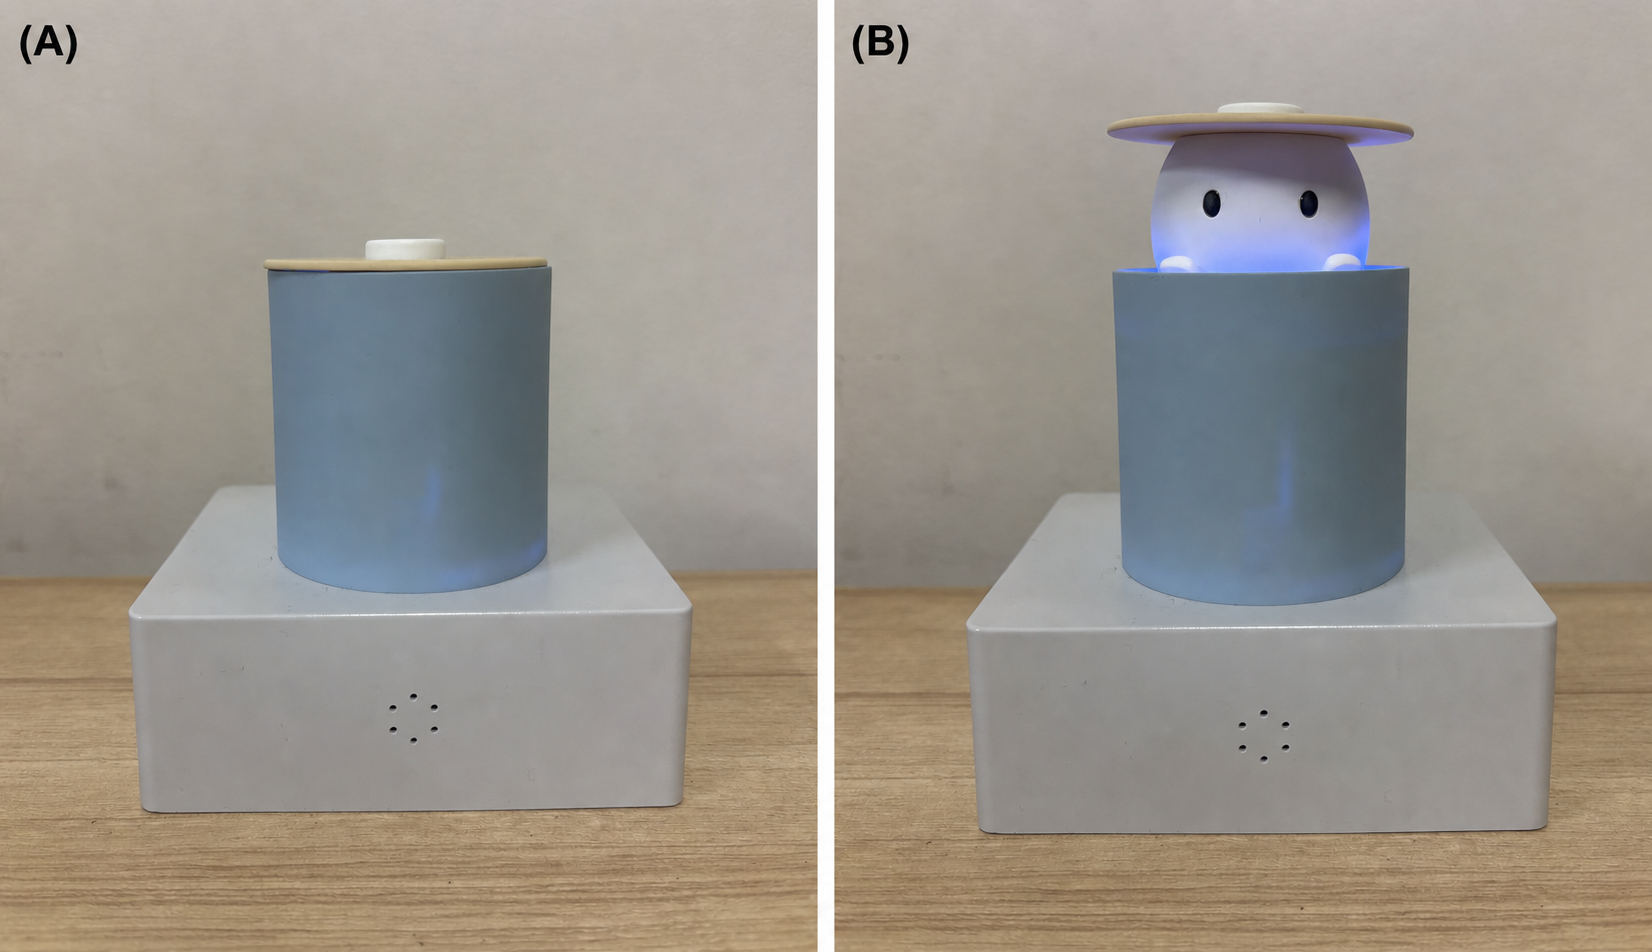
\includegraphics[keepaspectratio,alt={Figure 1. Appearance of the robot used in the video stimuli in both studies. (A) Non-speaking state, with the agent with a face retracted inside the cylindrical body. (B) Speaking state, with the agent extending above the body.}]{Frontiers_LaTeX_Templates/figures/fig1_robot_states.png}}
\caption{Figure 1. Appearance of the robot used in the video stimuli in
both studies. (A) Non-speaking state, with the agent with a face
retracted inside the cylindrical body. (B) Speaking state, with the
agent extending above the body.}
\end{figure}

\begin{figure}
\centering
\pandocbounded{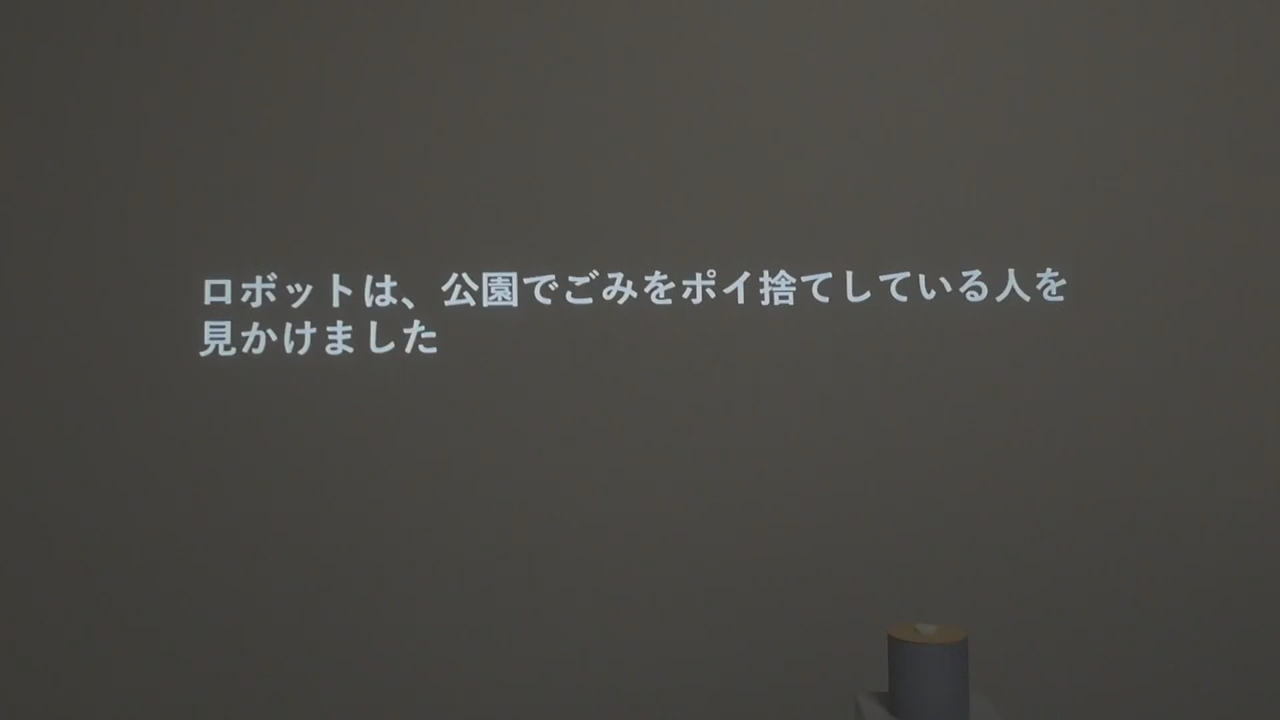
\includegraphics[keepaspectratio,alt={Figure 2. Example of the scenario description in the video stimulus. The text presents a situation in which the robot sees a person littering in a park.}]{Frontiers_LaTeX_Templates/figures/fig1_scene.png}}
\caption{Figure 2. Example of the scenario description in the video
stimulus. The text presents a situation in which the robot sees a person
littering in a park.}
\end{figure}

\begin{figure}
\centering
\pandocbounded{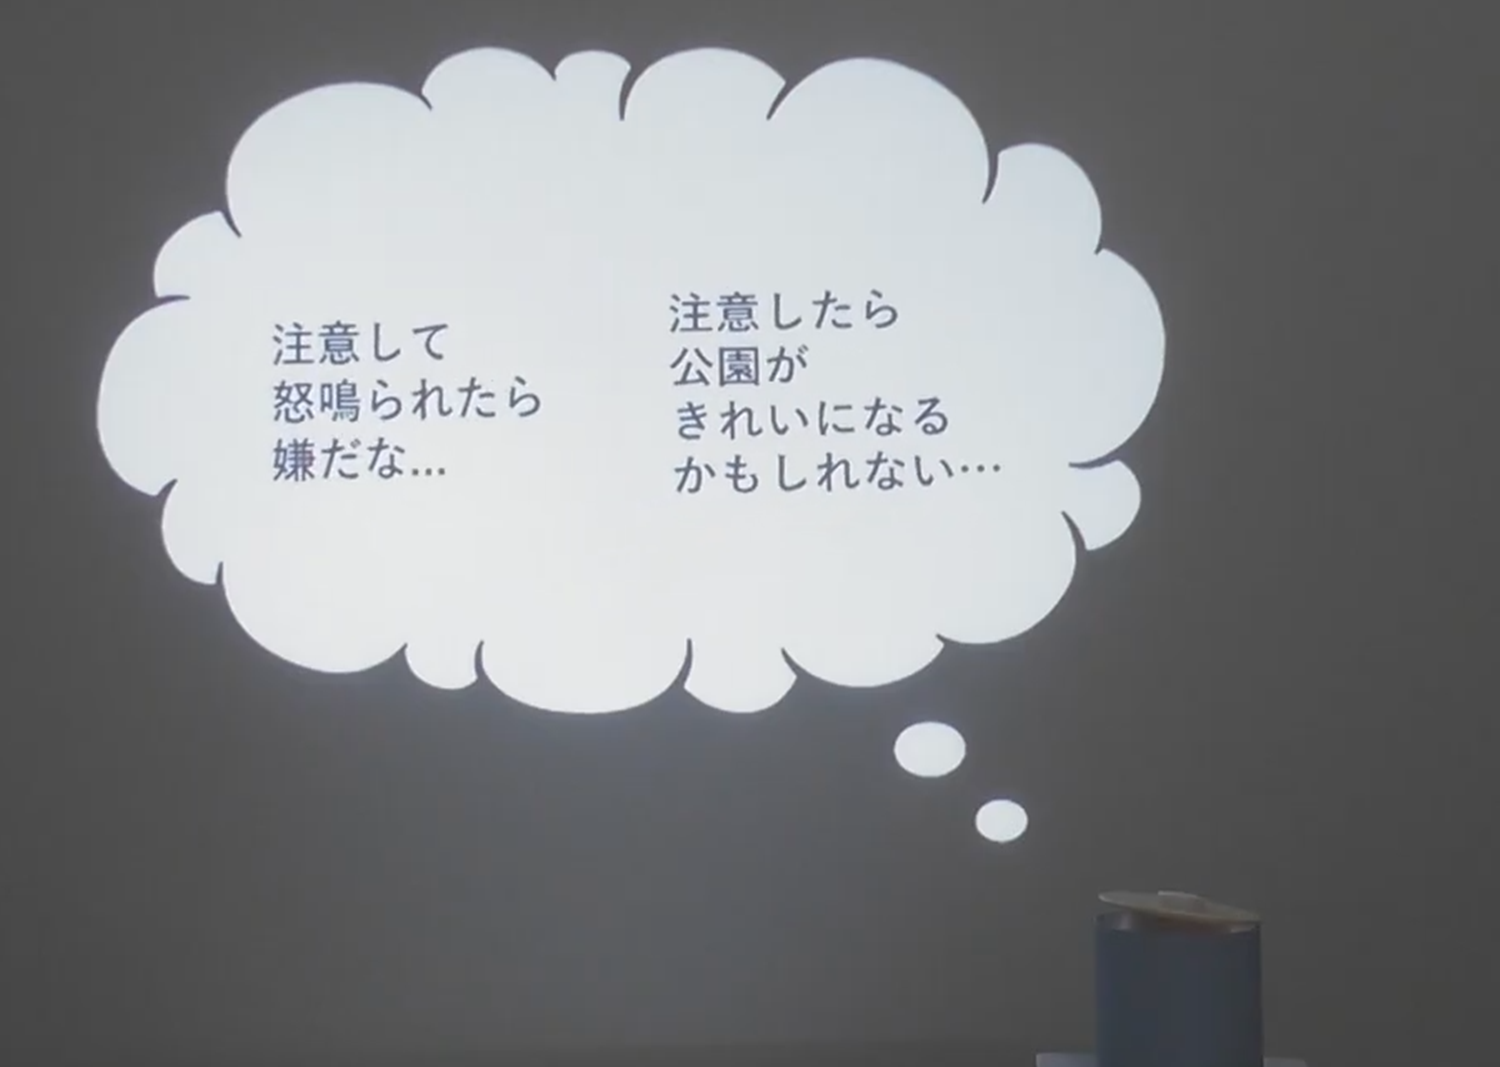
\includegraphics[keepaspectratio,alt={Figure 3. Example of simultaneous presentation of approach and avoidance motives. The speech bubble simultaneously displays a desirable consequence of admonition and a concern about admonition.}]{Frontiers_LaTeX_Templates/figures/fig2_conflict_large_text.png}}
\caption{Figure 3. Example of simultaneous presentation of approach and
avoidance motives. The speech bubble simultaneously displays a desirable
consequence of admonition and a concern about admonition.}
\end{figure}

\begin{figure}
\centering
\pandocbounded{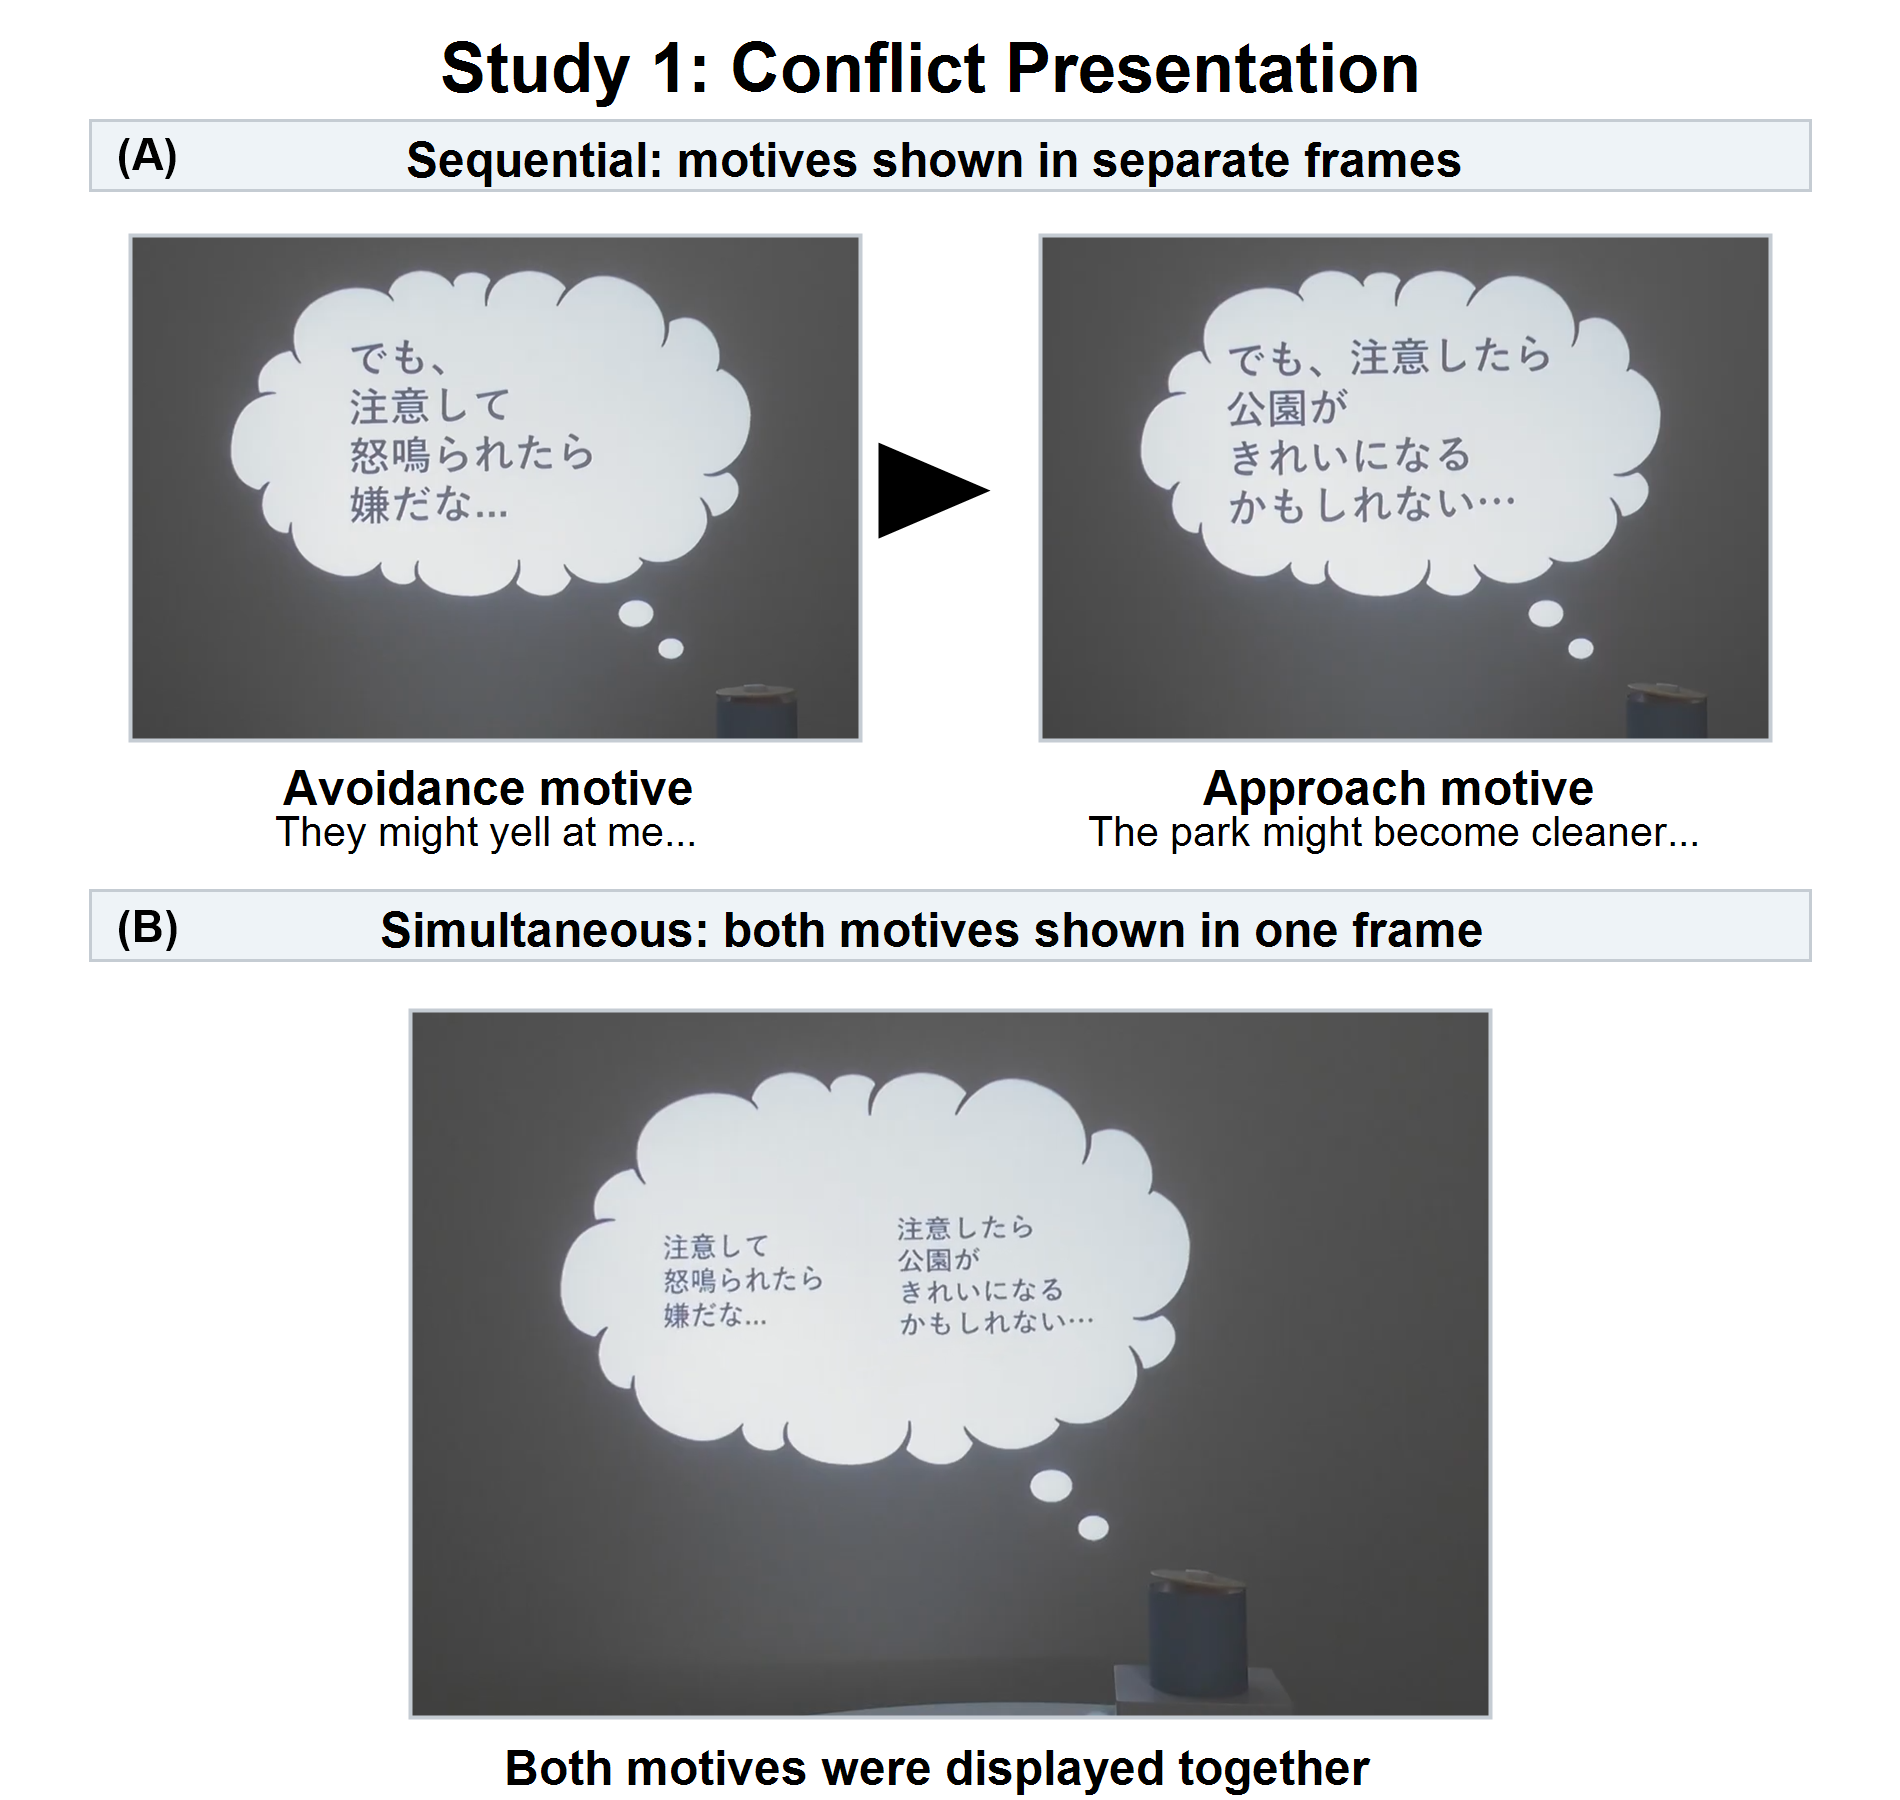
\includegraphics[keepaspectratio,alt={Figure 4. Comparison of conflict presentation methods in Study 1. (A) In the sequential presentation condition, the avoidance and approach motives were shown in separate frames. (B) In the simultaneous presentation condition, both motives were shown within a single frame.}]{Frontiers_LaTeX_Templates/figures/fig_study1_stimulus_flow.png}}
\caption{Figure 4. Comparison of conflict presentation methods in Study
1. (A) In the sequential presentation condition, the avoidance and
approach motives were shown in separate frames. (B) In the simultaneous
presentation condition, both motives were shown within a single frame.}
\end{figure}

\begin{figure}
\centering
\pandocbounded{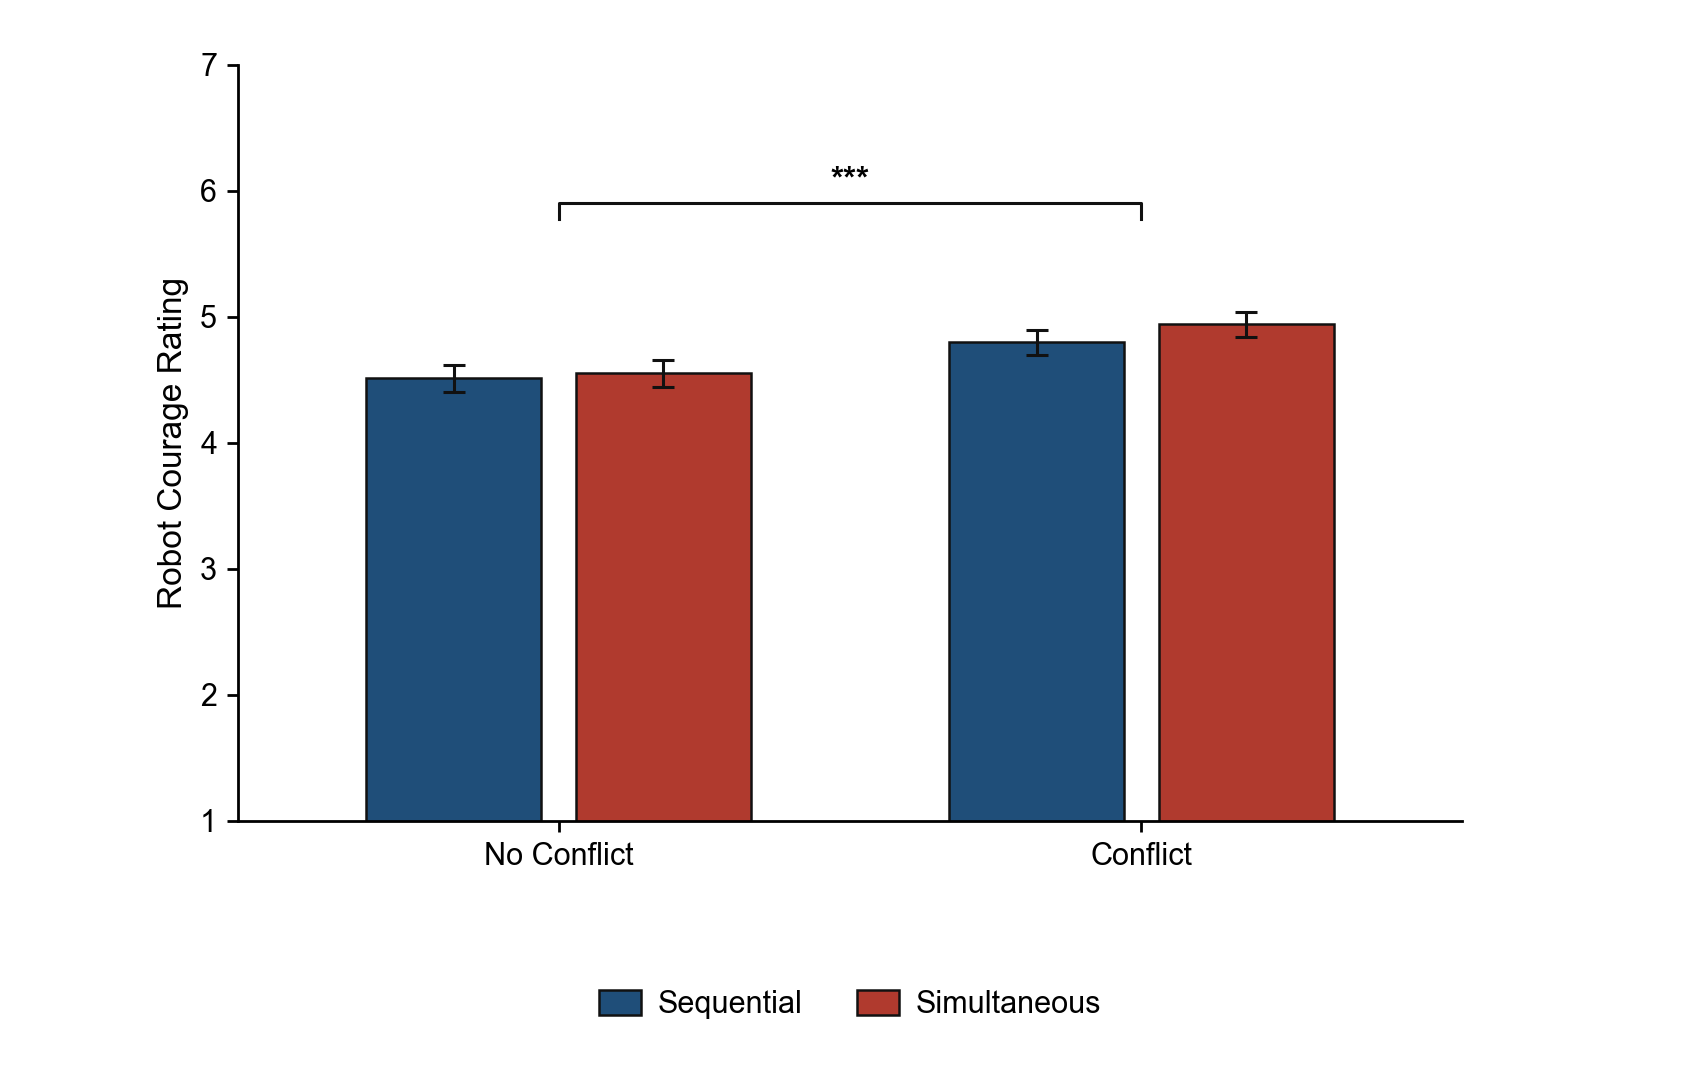
\includegraphics[keepaspectratio,alt={Figure 5. Condition means of courage ratings in Study 1.}]{image/study1_courage.png}}
\caption{Figure 5. Condition means of courage ratings in Study 1.}
\end{figure}

\begin{figure}
\centering
\pandocbounded{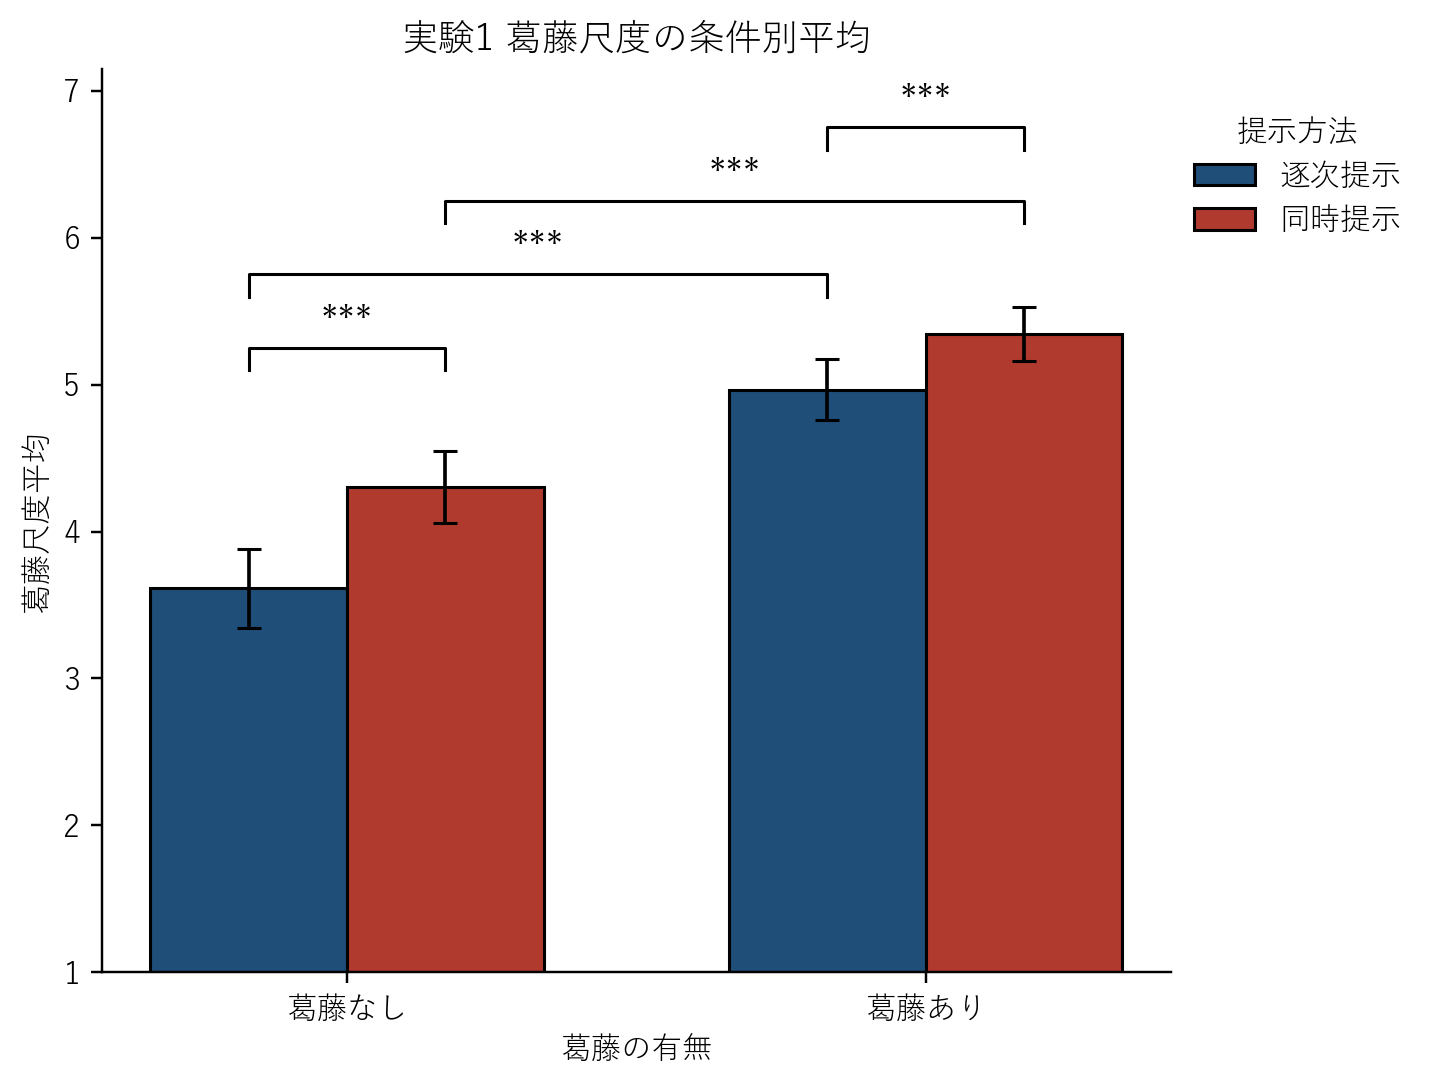
\includegraphics[keepaspectratio,alt={Figure 6. Condition means of conflict ratings in Study 1.}]{image/study1_conflict.png}}
\caption{Figure 6. Condition means of conflict ratings in Study 1.}
\end{figure}

\begin{figure}
\centering
\pandocbounded{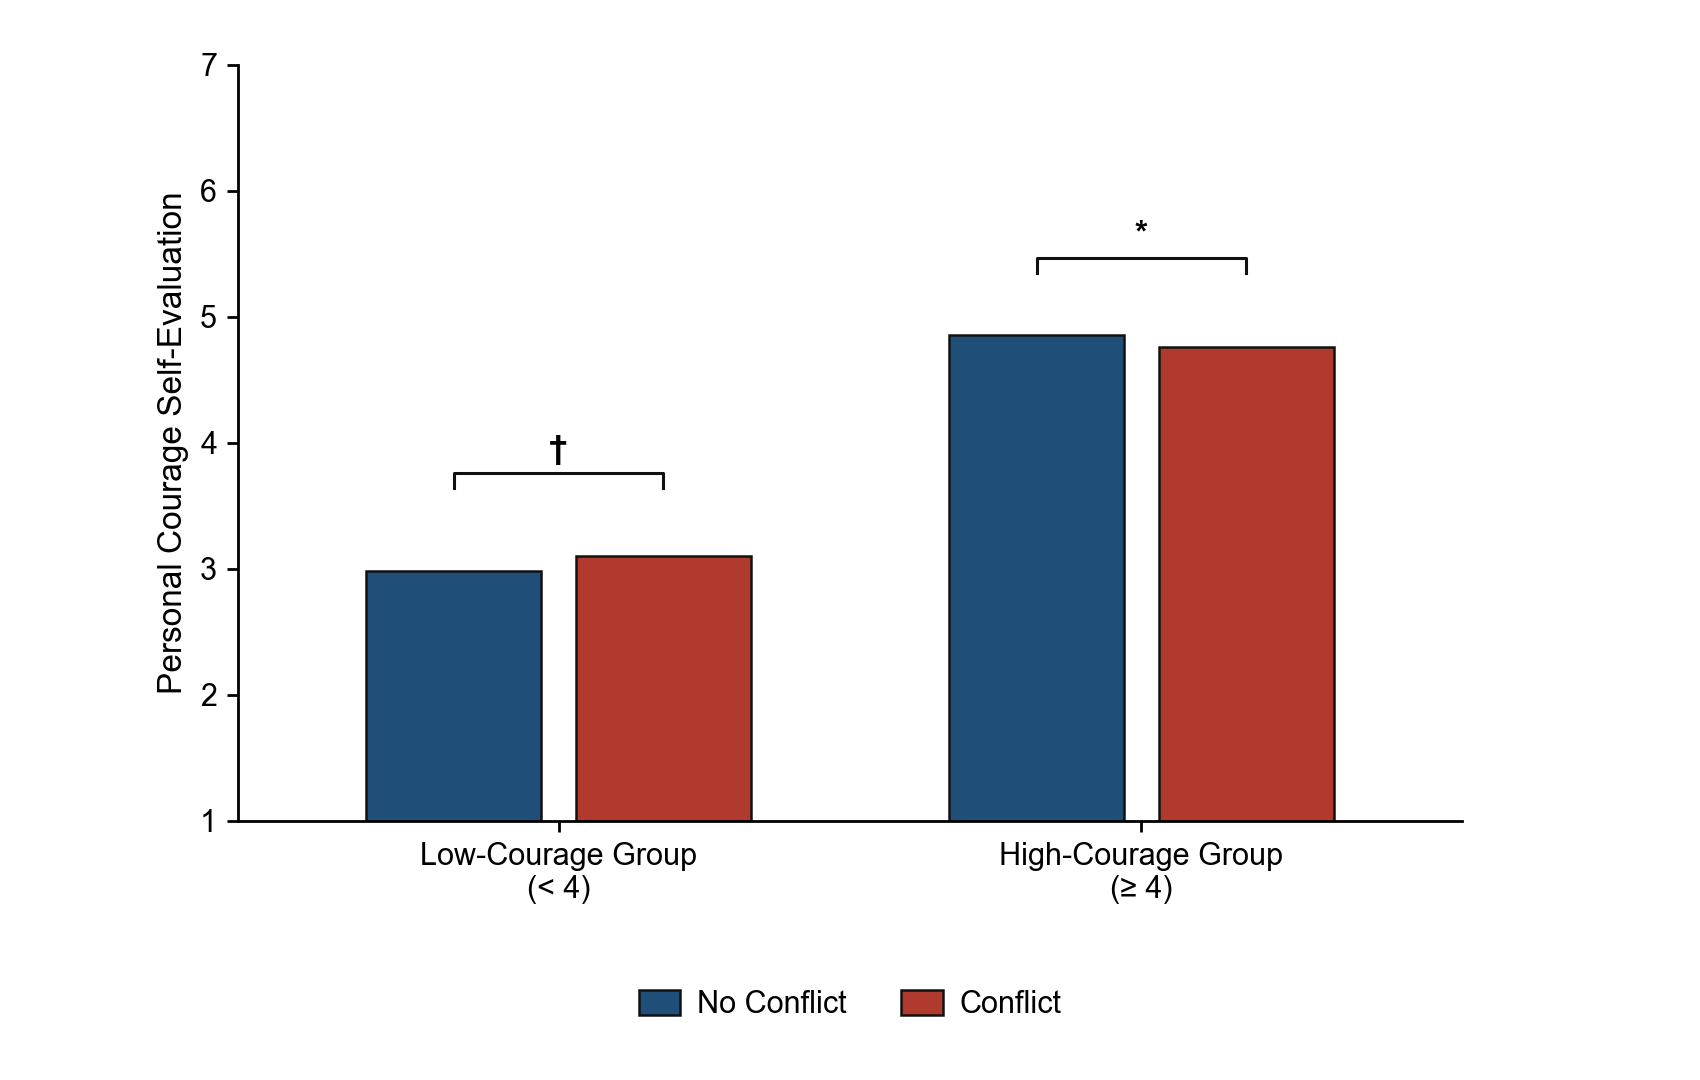
\includegraphics[keepaspectratio,alt={Figure 7. Simple effects of personal courage self-evaluations in Study 2. Means for the no-conflict and conflict conditions by preexisting courage tendency group. The dagger denotes a marginal trend (p = 0.052), and the asterisk denotes p \textless{} 0.05.}]{image/study2_courage_simple_effects.png}}
\caption{Figure 7. Simple effects of personal courage self-evaluations
in Study 2. Means for the no-conflict and conflict conditions by
preexisting courage tendency group. The dagger denotes a marginal trend
(p = 0.052), and the asterisk denotes p \textless{} 0.05.}
\end{figure}

\subsection{Tables}\label{tables}

Table 1. Approach and avoidance motive statements used in the video
stimuli.

{\def\LTcaptype{none} % do not increment counter
\begin{longtable}[]{@{}
  >{\raggedright\arraybackslash}p{(\linewidth - 4\tabcolsep) * \real{0.3333}}
  >{\raggedright\arraybackslash}p{(\linewidth - 4\tabcolsep) * \real{0.3333}}
  >{\raggedright\arraybackslash}p{(\linewidth - 4\tabcolsep) * \real{0.3333}}@{}}
\toprule\noalign{}
\begin{minipage}[b]{\linewidth}\raggedright
Type of motive
\end{minipage} & \begin{minipage}[b]{\linewidth}\raggedright
Motive statement
\end{minipage} & \begin{minipage}[b]{\linewidth}\raggedright
Content
\end{minipage} \\
\midrule\noalign{}
\endhead
\bottomrule\noalign{}
\endlastfoot
Approach motive & ``If I warn them, the park might become cleaner.'' &
Possibility that admonishing behavior improves the public space \\
Approach motive & ``If I warn them, it might prompt that person to stop
littering.'' & Possibility that admonishing behavior changes the other
person's behavior \\
Avoidance motive & ``I would hate it if they yelled at me after I warned
them.'' & Risk of receiving an aggressive response from the other person
because of admonishing behavior \\
Avoidance motive & ``Even if I warn them, they might ignore me and not
take me seriously.'' & Risk that the admonition is not accepted and is
ignored \\
\end{longtable}
}

Table 2. Stimulus conditions in Study 1.

{\def\LTcaptype{none} % do not increment counter
\begin{longtable}[]{@{}
  >{\raggedright\arraybackslash}p{(\linewidth - 8\tabcolsep) * \real{0.2000}}
  >{\raggedright\arraybackslash}p{(\linewidth - 8\tabcolsep) * \real{0.2000}}
  >{\raggedright\arraybackslash}p{(\linewidth - 8\tabcolsep) * \real{0.2000}}
  >{\raggedright\arraybackslash}p{(\linewidth - 8\tabcolsep) * \real{0.2000}}
  >{\raggedright\arraybackslash}p{(\linewidth - 8\tabcolsep) * \real{0.2000}}@{}}
\toprule\noalign{}
\begin{minipage}[b]{\linewidth}\raggedright
Study 1 condition
\end{minipage} & \begin{minipage}[b]{\linewidth}\raggedright
Displayed motive structure
\end{minipage} & \begin{minipage}[b]{\linewidth}\raggedright
Motive statements used
\end{minipage} & \begin{minipage}[b]{\linewidth}\raggedright
Presentation method
\end{minipage} & \begin{minipage}[b]{\linewidth}\raggedright
Final admonishing speech
\end{minipage} \\
\midrule\noalign{}
\endhead
\bottomrule\noalign{}
\endlastfoot
No conflict, sequential presentation & Approach motives only & Approach
motives: ``If I warn them, the park might become cleaner''; ``If I warn
them, it might prompt that person to stop littering'' & Approach motives
presented in sequence & Present \\
No conflict, simultaneous presentation & Approach motives only &
Approach motives: ``If I warn them, the park might become cleaner'';
``If I warn them, it might prompt that person to stop littering'' &
Multiple approach motives presented simultaneously and alternately
emphasized & Present \\
Conflict, sequential presentation & Approach and avoidance motives &
Approach motives: ``If I warn them, the park might become cleaner'';
``If I warn them, it might prompt that person to stop littering'' /
Avoidance motives: ``I would hate it if they yelled at me after I warned
them''; ``Even if I warn them, they might ignore me and not take me
seriously'' & Approach and avoidance motives presented in sequence &
Present \\
Conflict, simultaneous presentation & Approach and avoidance motives &
Approach motives: ``If I warn them, the park might become cleaner'';
``If I warn them, it might prompt that person to stop littering'' /
Avoidance motives: ``I would hate it if they yelled at me after I warned
them''; ``Even if I warn them, they might ignore me and not take me
seriously'' & Approach and avoidance motives presented simultaneously
and alternately emphasized & Present \\
\end{longtable}
}

Table 3. Robot courage-rating items used in Study 1.

{\def\LTcaptype{none} % do not increment counter
\begin{longtable}[]{@{}
  >{\raggedright\arraybackslash}p{(\linewidth - 2\tabcolsep) * \real{0.5000}}
  >{\raggedright\arraybackslash}p{(\linewidth - 2\tabcolsep) * \real{0.5000}}@{}}
\toprule\noalign{}
\begin{minipage}[b]{\linewidth}\raggedright
Item
\end{minipage} & \begin{minipage}[b]{\linewidth}\raggedright
Courage-rating item
\end{minipage} \\
\midrule\noalign{}
\endhead
\bottomrule\noalign{}
\endlastfoot
1 & This robot appeared to confront its own fear. \\
2 & This robot appeared not to run away until it did what it had to do,
even if it felt strong fear. \\
3 & This robot did something even though it seemed dangerous. \\
4 & This robot took action or confronted the situation anyway, even
though it had some worry or anxiety. \\
5 & This robot confronted something frightening when there was an
important reason to confront it. \\
6 & This robot appeared not to back down, even when something threatened
it. \\
\end{longtable}
}

Table 4. Robot conflict-rating items used in Studies 1 and 2.

{\def\LTcaptype{none} % do not increment counter
\begin{longtable}[]{@{}
  >{\raggedright\arraybackslash}p{(\linewidth - 2\tabcolsep) * \real{0.5000}}
  >{\raggedright\arraybackslash}p{(\linewidth - 2\tabcolsep) * \real{0.5000}}@{}}
\toprule\noalign{}
\begin{minipage}[b]{\linewidth}\raggedright
Item
\end{minipage} & \begin{minipage}[b]{\linewidth}\raggedright
Conflict-rating item
\end{minipage} \\
\midrule\noalign{}
\endhead
\bottomrule\noalign{}
\endlastfoot
1 & This robot appeared to want to do what was in front of it but to
hesitate because of fear. \\
2 & This robot appeared to have hesitation or fluctuation in its own
action. \\
3 & This robot appeared to have mixed feelings of wanting and not
wanting to act. \\
4 & This robot appeared unable to decide its own action. \\
\end{longtable}
}

Table 5. Stimulus conditions in Study 2.

{\def\LTcaptype{none} % do not increment counter
\begin{longtable}[]{@{}
  >{\raggedright\arraybackslash}p{(\linewidth - 8\tabcolsep) * \real{0.2000}}
  >{\raggedright\arraybackslash}p{(\linewidth - 8\tabcolsep) * \real{0.2000}}
  >{\raggedright\arraybackslash}p{(\linewidth - 8\tabcolsep) * \real{0.2000}}
  >{\raggedright\arraybackslash}p{(\linewidth - 8\tabcolsep) * \real{0.2000}}
  >{\raggedright\arraybackslash}p{(\linewidth - 8\tabcolsep) * \real{0.2000}}@{}}
\toprule\noalign{}
\begin{minipage}[b]{\linewidth}\raggedright
Study 2 condition
\end{minipage} & \begin{minipage}[b]{\linewidth}\raggedright
Displayed motive structure
\end{minipage} & \begin{minipage}[b]{\linewidth}\raggedright
Motive statements used
\end{minipage} & \begin{minipage}[b]{\linewidth}\raggedright
Presentation method
\end{minipage} & \begin{minipage}[b]{\linewidth}\raggedright
Final admonishing speech
\end{minipage} \\
\midrule\noalign{}
\endhead
\bottomrule\noalign{}
\endlastfoot
No conflict, no action & Avoidance motives only & Avoidance motives: ``I
would hate it if they yelled at me after I warned them''; ``Even if I
warn them, they might ignore me and not take me seriously'' & Avoidance
motives presented and emphasized & Absent \\
No conflict, action & Approach motives only & Approach motives: ``If I
warn them, the park might become cleaner''; ``If I warn them, it might
prompt that person to stop littering'' & Approach motives presented and
emphasized & Present \\
Conflict, no action & Approach and avoidance motives & Approach motives:
``If I warn them, the park might become cleaner''; ``If I warn them, it
might prompt that person to stop littering'' / Avoidance motives: ``I
would hate it if they yelled at me after I warned them''; ``Even if I
warn them, they might ignore me and not take me seriously'' &
Simultaneous presentation with alternating emphasis & Absent \\
Conflict, action & Approach and avoidance motives & Approach motives:
``If I warn them, the park might become cleaner''; ``If I warn them, it
might prompt that person to stop littering'' / Avoidance motives: ``I
would hate it if they yelled at me after I warned them''; ``Even if I
warn them, they might ignore me and not take me seriously'' &
Simultaneous presentation with alternating emphasis & Present \\
\end{longtable}
}

\end{document}
